\documentclass{article}
\usepackage[a4paper, total={6in, 8in}]{geometry}
\usepackage{algorithm}
\usepackage{algorithmic}
\usepackage{amsmath}
\usepackage{amssymb}
\usepackage{amsfonts}
\usepackage{bbm}
\usepackage{blindtext}
\usepackage{caption}
\usepackage{cancel}
\usepackage{color}
\usepackage{epstopdf}
\usepackage{etoolbox}
\usepackage{float}
\usepackage{graphicx}
\usepackage{hyperref}
\usepackage{multirow}
\usepackage{pgfplots}
\usepackage{tikz}
\usepackage{url}
\usepackage{times}
\usepackage{tkz-graph}
\usepackage[np]{numprint} 
\usepackage{verbatim}  
\usepackage{multicol}
\usepackage{threeparttable}
\usepackage{subcaption}
\usepackage{listings}
\usepackage{tkz-euclide}
\usepackage{stackengine}
\usepackage{enumitem}


\usetikzlibrary{calc}
\usetikzlibrary{fit}
\usetikzlibrary{arrows}
\usetikzlibrary{backgrounds}
\usetikzlibrary{shapes}
\usetikzlibrary{positioning}
\usetikzlibrary{decorations.pathmorphing}
\usetikzlibrary{decorations.pathreplacing}
\usetikzlibrary{decorations.markings}
\usetikzlibrary{arrows.meta}


\def\L{\mathcal{L}}
\def\E{\mathbb{E}}
\def\N{\mathcal{N}}
\def\KL{\mathbb{KL}}
\def\d{\text{d}}
\def\ep{{\epsilon}}
\def\VAR{\mathbb{VAR}}
\def\COV{\mathbb{COV}}

\def\a{{\mathbf a}}
\def\b{{\mathbf b}}
\def\c{{\mathbf c}}
%\def\d{{\mathbf d}}
\def\e{{\mathbf e}}
\def\f{{\mathbf f}}
\def\g{{\mathbf g}}
\def\h{{\mathbf h}}
\def\i{{\mathbf i}}
\def\j{{\mathbf j}}
\def\k{{\mathbf k}}
\def\l{{\mathbf l}}
\def\m{{\mathbf m}}
\def\n{{\mathbf n}}
\def\o{{\mathbf o}}
\def\p{{\mathbf p}}
\def\q{{\mathbf q}}
\def\r{{\mathbf r}}
\def\s{{\mathbf s}}
\def\t{{\mathbf t}}
\def\u{{\mathbf u}}
\def\v{{\mathbf v}}
\def\w{{\mathbf w}}
\def\x{{\mathbf x}}
\def\y{{\mathbf y}}
\def\z{{\mathbf z}}



\def\A{{\mathbf A}}
\def\B{{\mathbf B}}
\def\C{{\mathbf C}}
\def\D{{\mathbf D}}
%\def\E{{\mathbf E}}
\def\F{{\mathbf F}}
\def\G{{\mathbf G}}
\def\H{{\mathbf H}}
\def\I{{\mathbf I}}
\def\J{{\mathbf J}}
\def\K{{\mathbf K}}
%\def\L{{\mathbf L}}
\def\M{{\mathbf M}}
%\def\N{{\mathbf N}}
\def\O{{\mathbf O}}
\def\P{{\mathbf P}}
\def\Q{{\mathbf Q}}
\def\R{{\mathbf R}}
\def\S{{\mathbf S}}
\def\T{{\mathbf T}}
\def\U{{\mathbf U}}
\def\V{{\mathbf V}}
\def\W{{\mathbf W}}
\def\X{{\mathbf X}}
\def\Y{{\mathbf Y}}
\def\Z{{\mathbf Z}}

\def\0{{\bf 0}}
\def\1{{\mathbbm{1}}}
\def\Rad{\text{Rad}_n(\H)}
\def\RadE{\widehat{\text{Rad}}_S(\H)}
\def\RadF{\text{Rad}_n(\F)}
\def\aalpha{\boldsymbol{\alpha}}
\def\bbeta{\boldsymbol{\beta}}
\def\ggamma{\boldsymbol{\gamma}}
\def\eeta{\boldsymbol{\eta}}
\def\eepsilon{\boldsymbol{\epsilon}}
\def\llambda{\boldsymbol{\lambda}}
\def\ssigma{\boldsymbol{\sigma}}
\def\pphi{\boldsymbol{\phi}}
\def\ppi{\boldsymbol{\pi}}
\def\ppi{\boldsymbol{\mmu}}
\def\ttheta{\boldsymbol{\theta}}
\def\ddelta{\boldsymbol{\delta}}
\def\GGamma{{\boldsymbol{\Gamma}}}

\def\PR{{p_{\text{r}}}}
\def\PG{{p_{\text{g}}}}

\def\na{{\nabla}}

\newtheorem{definition}{Definition}
\newtheorem{theorem}{Theorem}
\newtheorem{lemma}{Lemma}
\newtheorem{proposition}{Proposition}
\newtheorem{conjecture}{Conjecture}
\newtheorem{example}{Example}
\newtheorem{property}{Property}
\newtheorem{comments}{Comments}
\newtheorem{remark}{Remark}


\DeclareMathOperator*{\argmin}{arg\,min}
\DeclareMathOperator*{\argmax}{arg\,max}

\def\delequal{\mathrel{\ensurestackMath{\stackon[1pt]{=}{\scriptstyle\Delta}}}}
\def\Dtheta{{\triangledown_\theta}}
\def\NT{{\nabla_\theta}}

\def\optional{{\color{red} Optional - not examinable}}

\def\exam{{\color{blue} High chance to be examined}}

\def\prox{{\text{prox}}}


\newlist{Properties}{enumerate}{2}
\setlist[Properties]{label=Property \arabic*., font=\textbf, itemindent=*}
\graphicspath{{images/}}

\def\DLambda{\nabla_{\lambda}}
\def\DPhi{\nabla_{\phi_{n,j}}}
\def\post{\text{post}}
\def\pri{\text{pri}}
\def\Optional{}
%\def\Optional{\color{red}Optional for Exam}
\def\OC{\color{white}}

\def\C{\text{Const.}}
%\def\NT{{\nabla_\theta}}
%\def\BT{{\bf{\theta}}}
%\def\COV{{\mathbf{Cov}}}
%\def\Var{\mathbb{VAR}}
%\def\SIGMA{{\boldsymbol {\Sigma }}}
%\newcommand{\tens}[1]{
%  \mathbin{\mathop{\otimes}\limits_{#1}}
%}
%
%\def\bx{{\mathbf x}}
%\def\bw{{\mathbf w}}
%\def\bz{{\mathbf z}}
%\def\BT{\boldsymbol\theta}
%\def\layersep{2.5cm}
%\def\predone{{{\bf attribute 1}}}
%\def\predtwo{{{\bf attribute 2}}}
%\def\predthree{{{\bf attribute 3}}}
%\def\tanh{{\text{tanh}}}
%\def\x{{\mathbf x}}
%\def\w{{\mathbf w}}
%\def\N{{\mathcal{N}}}
%\def\L{{\cal L}}
%\def\PHI{{\Phi }}
%\def\offset{b}
%\def\BY{{\mathbf{Y}}}
%\def\bY{{\bf Y}}
%\def\Dtheta{{\nabla_\theta}}
%\def\PR{{p_{\text{r}}}}
%\def\PG{{p_{\text{g}}^\theta}}
%\definecolor{red}{rgb}{1.00,0.00,0.00}
%\definecolor{blue}{rgb}{0.00,0.00,1.00}
%\def\SIGMA{{\boldsymbol \Sigma}}
%\def\SIGMAH{{\boldsymbol \Sigma^{\frac{1}{2}}}}
%\def\Sigmah{{\Sigma^{\frac{1}{2}}}}
%\def\MU{\boldsymbol {\mu }}
%\def\EP{\boldsymbol {\ep }}
%\def\aalpha{\boldsymbol {\alpha }}
%\def\mark{\bf{\color{red} CHANGE}}
%\def\neww{\bf{\color{red} NEW}}
%\def\thetablue{{\color{blue} \bf {\theta}}}
%\def\NT{{\nabla_\theta}}
%\def\Policy{{\pi_\theta(a \vert s)}}
%\def\ep{{\epsilon}}
%\def\bpi{{\boldsymbol{\pi}}}
%
%\def\ga{{\text{ga}}}
%\def\GA{{\mathcal{G}\text{A}}}
%\def\GATR{{{\mathcal{G}\text{A}}_{\text{truncate}}}}
%\def\TZ{{\tilde{z}}}
%%\def\TZ{{z}}
%\def\Z{{\mathcal{Z}}}
%
%\def \Nbins{K}
%\def \Knew{k^{\text{new}}}
%\def \Tzmath{\mathcal{Z}}
%\def \Znji{{\bf z}^{-ji}}
%\def \Clm{{\bf C}_{l,m}}
%%\def \Alm{{\bf A}_{l,m}}
%\def \Alm{{\bf A}}
%\def\KL{\mathbb{KL}}
%\def\C{\text{const.}}
%\def\BETA{\beta}
%\def\qtheta{q_{\theta}(\theta)}
%\def\qZ{q_z(Z)}
%\def\1{\mathbbm{1}}
%
%\def\bbeta{\boldsymbol{\beta}}
%\def\aalpha{\boldsymbol{\alpha}}
%\def\eeta{\boldsymbol{\eta}}




\title{Variational Bayes}
\author{Richard Xu}

\begin{document}

\maketitle 


\section{Motivation}

We are now in the Artificial Intelligence Generated Content (AIGC) era. The goal of AIGC is to be able to sample from the data distribution $p(\x)$. For example, there may be a dataset of images $\mathcal{D}$; if we can build a distribution $p(\x)$ reflecting the training data, then we are able to generate new images that are similar to $\mathcal{D}$ by sampling from its distribution $p(\x)$.



To do so, we must be able to find out the parameterised distribution of $p_\theta(\x)$ first. However, we cannot possibly compute the distribution of $p(\x)$ over $\mathcal{D}$ or even assume what type of distribution it is. Therefore, we can only approximate it with simple (or simpler) distributions $q_\phi(\z)$, where $\phi$ are the parameters of the distribution.

\subsection{notation}

\begin{table}[h]
\centering
\begin{tabular}{|c|c|}
\hline
\textbf{Variable} & \textbf{Description} \\ \hline
$\x$ & Data point \\ \hline
$\mathcal{D} = \{\x_1, \dots, \x_n \}$ & Dataset \\ \hline
$p(\x)$ & Data distribution \\ \hline
$p_\theta(\x)$ & Parameterized data distribution \\ \hline
$q_\phi(\z)$ & Approximate distribution \\ \hline
$\phi$ & Parameters of the approximate distribution \\ \hline
$\z$ & Latent variable \\ \hline
$p(\z)$ & Prior distribution \\ \hline
$p(\x | \z)$ & Likelihood \\ \hline
$p(\z | \x)$ & Posterior distribution \\ \hline
$\KL(q\|p)$ & Kullback-Leibler divergence \\ \hline
$\text{ELBO}(q)$ & Evidence Lower Bound \\ \hline
$\mu$ & Mean of Gaussian distribution \\ \hline
$\tau$ & Precision (inverse of variance) \\ \hline
$\mu_0, \lambda_0$ & Prior (Gaussian) parameter for $\mu$\\ \hline
$a_0, b_0$ & Prior (Gamma) parameters for $\tau$ \\ \hline
$\mu_n, \lambda_n$ & Posterior (Gaussian) parameter for $\mu$ \\ \hline
$a_n, b_n$ & Posterior (Gamma) parameters for $\tau$ \\ \hline
$q_\mu(\mu)$ & Variational distribution for $\mu$ \\ \hline
$q_\tau(\tau)$ & Variational distribution for $\tau$ \\ \hline
\end{tabular}
\caption{List of Variables}
\label{tab:variables}
\end{table}

\subsection{a starting point}

However, let's start with a much simpler problem first. We assume that we know part of the information of the distribution $p(\x)$: the prior $p(\z)$ and the likelihood $p(\x | \z)$ (hence we also know the joint density $p(\x,\z)$). It appears that we also know the posterior distribution $p(\z | \x)$, as we can use Bayes' rule to compute the posterior distribution, i.e.,:

\begin{equation}\begin{split}
p(\z | \x) = \frac{\overbrace{p(\x | \z)}^{\text{known}}\; \overbrace{p(\z)}^{\text{known}}}{\underbrace{\int_{\z'} p(\x|\z') p(\z') \d \z'}_{\text{don't know analytically}} }
\end{split}\end{equation}

But unfortunately, we do not always have access to the posterior distribution in closed form.

Also in this section, we do not worry about learning the parameters $\theta$ associated with $p_\theta(\z | \x)$, which is something we will consider later for Variational Autoencoders (VAE).

\subsubsection{toy example}

to illustrate what is an observed data $\x$ and what is a latent space $\z$, let's look at the same ``student mark'' toy example you saw in both the probabilistic graphical models (which we will retrospectively visit again) and MCMC sections:

\begin{enumerate}
\item
``months of studies'' (stu)  $z_1$
\item
``prior knowledge'' (pkw) $z_2$
\item
``motivation'' (mot)  $z_3$
\item
``mark obtained'' (mrk) $\x$
\end{enumerate}

\begin{center}
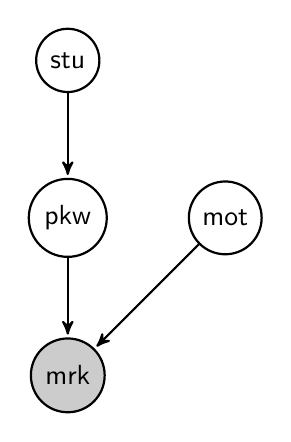
\begin{tikzpicture}[->,>=stealth',shorten >=1pt,auto,node distance=2.5cm,
	  thick,main node/.style={circle,draw,font=\sffamily\normalsize, minimum size = 3.5pt}]
	
	 \node[main node] (stu) {\text{stu}};
	 \node[main node] (pkw) at ($ (stu) + (270:2.0) $) {pkw};
	 \node[main node] (mot) at ($ (pkw) + (0:2.0) $) {\text{mot}};
	 \node[main node, fill=gray!40] (mrk) at ($ (pkw) + (270:2.0) $) {mrk};
	 \path[every node/.style={font=\sffamily\small}]
	    (stu) edge  (pkw)
	    (mot) edge  (mrk)
	    (pkw) edge  (mrk)
;
	\end{tikzpicture}
\end{center}

We have three latent variables, (stu), (pkw), (mot) and one observation (mrk). Then, if we want to perform posterior inference, i.e.,:

\begin{equation}\begin{split}
&\Pr \big(\underbrace{\text{stu},\text{pkw},\text{mot}}_{\text{latent}} | \underbrace{\text{mrk}}_{\text{observation}}\big)
\end{split}\end{equation}

which allows us to compute things such as:

\begin{equation}\begin{split}
&\E_{ \Pr \big(\text{stu},\text{pkw},\text{mot} | \text{mrk} \big)} [ \text{stu},\text{pkw},\text{mot}  ]
\end{split}\end{equation}

%Unlike Markov Chain Monte Carlo (MCMC), in variational inference, there is NO sampling, instead we propose a set of distributions, $q_{\phi_\text{stu}}(\text{stu})$, $q_{\phi_\text{pkw}}(\text{pkw})$ and $q_{\phi_\text{mot}}(\text{mot})$, such that the $\KL$ divergence between $q( \text{stu}, \text{pkw}, \text{mot}) = q_{\phi_\text{stu}}(\text{stu}) \times q_{\phi_\text{pkw}}(\text{pkw}) \times q_{\phi_\text{mot}}(\text{mot})$ and  $\Pr \big(\text{stu},\text{pkw},\text{mot} | \text{mrk} \big)$ are minimized!. Obviously, we need to optimize with respect with the parameters $\phi_\text{stu}$, $\phi_\text{pkw}$ and $\phi_\text{mot}$.


Unlike Markov Chain Monte Carlo (MCMC), in variational inference, instead of sampling, we propose a set of proposal distributions, $q_{\phi_\text{stu}}(\text{stu})$, $q_{\phi_\text{pkw}}(\text{pkw})$ and $q_{\phi_\text{mot}}(\text{mot})$ which aim to minimize the $\KL$ divergence between:


\begin{equation}\begin{split}
q(\text {stu}, \text{pkw}, \text{mot}) = q_{\phi_\text{stu}}(\text{stu}) \times q_{\phi_\text{pkw}}(\text{ pkw}) \times q_{\phi_\text{mot}}(\text{mot})
\end{split}\end{equation}

and 

\begin{equation}\begin{split}
\Pr \big(\underbrace{\text{stu}}_{z_1},\underbrace{\text{pkw}}_{z_2},\underbrace{\text{mot}}_{z_3} | \underbrace{\text {mrk}}_{\x} \big)\\
\end{split}\end{equation}

Obviously, we need to optimize with respect to the parameters $\phi_\text{stu}$, $\phi_\text{pkw}$ and $\phi_\text{mot}$. Then after that one can approximate:

\begin{equation}\begin{split}
\E_{ \Pr \big(\text{stu},\text{pkw},\text{mot} | \text{mrk} \big)} [ \text{stu},\text{pkw},\text{mot}  ]
\approx \E_{ q \big(\text{stu},\text{pkw},\text{mot} \big)} [ \text{stu},\text{pkw},\text{mot}  ]
\end{split}\end{equation}



\subsubsection{LDA example \optional}


For example, in the LDA example:

\begin{equation}\begin{split}
\text{observation:}\quad &\{ w_{d \in \{1 \dots D \}, n \in \{1 \dots N \}  } \}  \\
\text{latent variable:}\quad &\{ \{ \bbeta_j \}_{j=1}^K ,  \{\ttheta_d\}_{d=1}^D,  \{ z_{d \in \{1 \dots D \}, n \in \{1 \dots N \} } \} \}
\end{split}\end{equation}

Therefore, in LDA, the variational inference aims to:

\begin{equation}\begin{split}
&p \Big(  \{ \bbeta_j \}_{j=1}^K ,  \{\ttheta_d\}_{d=1}^D,  \{ z_{d \in \{1 \dots D \}, n \in \{1 \dots N \} } \} \big|  
\{ w_{d \in \{1 \dots D \}, n \in \{1 \dots N \} } \} \Big)\\
&\approx \prod_{j=1}^K q(\bbeta_j | \llambda_j) \prod_{d=1}^D q(\ttheta_d | \ggamma_d) \prod_{d=1}^D \prod_{n=1}^N q(z_{d,n} | \pphi_{d,n})
\end{split}\end{equation}

it allows us to approximate:

\begin{equation}\begin{split}
\E_p \Big[ \Big\{ \{ \bbeta_j \}_{j=1}^K ,  \{\ttheta_d\}_{d=1}^D,  \{ z_{d \in \{1 \dots D \}, n \in \{1 \dots N \} } \}\Big\} \Big]
\approx
\E_q \Big[ \Big\{ \{ \bbeta_j \}_{j=1}^K ,  \{\ttheta_d\}_{d=1}^D,  \{ z_{d \in \{1 \dots D \}, n \in \{1 \dots N \} } \}\Big\} \Big]
\end{split}\end{equation}

we just need to optimize with respect to $\{  \llambda_j \}, \{ \ggamma_d \}, \{  \pphi_{d,n} \} $

\subsection{A bit of history \dots}

This note started in 2010 when I was inspired to help people read Chapter 10 of Bishop \cite{bishop2006pattern} where I was trying to explain a few things in an oversimplified (hopefully!) way. I later revamped it. I also added exponential family distributions and an example on LDA when the model is fully conjugate \cite{hoffman2013stochastic}.

\section{The Variational Bayes Framework}

Now imagine we have some training data for us to compute the distribution of it, i.e., $p(\x)$. Imagine we are able to compute its analytical form, then we can just sample from it, i.e., to create new data. However, in many cases, the distribution is intractable, i.e., we cannot compute it. Therefore, we need to approximate it.

Now, let's consider the following:

\subsection{what is the Evidence Lower Bound?}

\subsection{use Jensen's Inequality}


\begin{equation}\begin{split}
\log  p(\x) &= \log \int_{\z}  p(\x,\z)\d \z \\
&= \log \int_{\z} \frac{ p(\x,\z)}{q_{\phi}(\z|\x)} q_{\phi}(\z|\x) \d \z\\
&= \log \left[ \E_{z \sim q_{\phi}(\z|\x)} \left(\frac{ p(\x,\z)}{q_{\phi}(\z|\x)} \right) \right]\\
&\ge \E_{z \sim q_{\phi}(\z|\x)} \left[ \log  \left( \frac{ p(\x,\z)}{q_{\phi}(\z|\x)} \right) \right]\quad\quad\text{by Jensen's inequality}\\
&= \E_{z \sim q_{\phi}(\z|\x)} \left[ \log (  p(\x,\z) ) \right]  -
\E_{z \sim q_{\phi}(\z|\x)} \left[ \log ( q_{\phi}(\z|\x) ) \right]\\
&= \text{ELBO}(q)\\
\end{split}\end{equation}

\subsection{another expansion}

the above does not show what the missing bit $\log p(\x) - \text{ELBO}(q)$ is. So what is it?

\begin{equation}\begin{split}
\log{(p(\x))} &=  \log{  \left( \frac{p(\x,\z)}{p(\z|\x)} \right)  } \\
&=  \log{ (p(\x,\z)) } - \log{ (p(\z|\x)) }\\
&=  [ \log{ (p(\x,\z)) } - \log q_\phi(\z)] - [ \log{ (p(\z|\x)) } - \log q_\phi(\z)] \quad\quad \because \pm q_\phi(\z)\\
&=  \log{  \left(   \frac{p(\x,\z)}{q_\phi(\z)}  \right)  } -  \log{  \left(   \frac{p(\z|\x)}{q_\phi(\z)}  \right)  }\\
\end{split}\end{equation}


now, let's take the expectation on both sides, given $q_\phi(\z)$:



\begin{equation}\begin{split}
\log{(p(\x))} &=   \int q_\phi(\z) \log{  \left(   \frac{p(\x,\z)}{q_\phi(\z)}  \right)  } \d \z -  \int q_\phi(\z) \log{  \left(   \frac{p(\z|\x)}{q_\phi(\z)}  \right)  } \d \z\\
&=   \int q_\phi(\z) \log{  \left(   \frac{p(\x,\z)}{q_\phi(\z)}  \right)  } \d \z + \int q_\phi(\z) \log{  \left(   \frac{q_\phi(\z)}{p(\z|\x)}  \right)  } \d \z\\
&= \text{ELBO}(q) + \KL(q\|p)
\end{split}\end{equation}



\subsubsection{names for both terms}

\begin{equation}\begin{split}
\text{ELBO}(q) &= \int q_\phi(\z) \log{  \left(   \frac{p(\x,\z)}{q_\phi(\z)}  \right)  } \d \z
= \E_{z \sim q_\phi(\z) } \big[ \log \left(   \frac{p(\x,\z)}{q_\phi(\z)}  \right) \big]\\
\KL(q\|p) &= \int q_\phi(\z) \log{  \left(   \frac{q_\phi(\z)}{p(\z|\x)}  \right)  } \d \z 
\end{split}\end{equation}


now we can answer the question of why we do not minimize the $\KL$ term directly. The {\bf key} is that the $\KL$ term contains $p(\z | \x)$ and the ELBO term contains $p(\x|\z) p(\z)$! Why is this a problem? Because then one has to compute:


\begin{equation}\begin{split}
p(\x) = \int_{\z'} p(\x | \z') p(\z') \d \z'
\end{split}\end{equation}


%some may consider this isn't going to be a problem, as $p(\x)$ is just a constant. However, it's still dependa on the hypermaramter $\phi$, i.e.,:
%
%\begin{equation}\begin{split}
%\Big( p_{\phi_1}(x) = \int_{z'} p(x | z') p_{\phi_1}(z') \d \z' \Big)  \ne  \Big( p_{\phi_2}(x) = \int_{z'} p(x | z') p_{\phi_2}(z') \d \z'  \Big)
%\end{split}\end{equation}



%Now here comes the trick part: let's consider that $p(\x)$ is fixed with respect to the choice of $q_\phi(\z)$. We wanted to choose a $q_\phi(\z)$ function that minimize KL divergence, so that $q_\phi(\z)$ becomes closer and closer to $p(\z|\x)$. Of course, let's see what happens when $q_\phi(\z) = p(\z|\x)$:

since we can choose any $q_\phi(\z)$ we'd like, and since we want $\KL(\cdot)$ to be minimized, it is ideal to make:

\begin{equation}\begin{split}
q_\phi(\z) \equiv q_\phi(\z|\x)
\end{split}\end{equation}

i.e., it should also depend on $\x$. Otherwise, it's highly unlikely that the $ \KL \big(q\|p(\z|\x) \big) $ will be minimized:


\begin{equation}\begin{split}
 \KL(q\|p) = \int q_\phi(\z|\x) \log{  \left(   \frac{q_\phi(\z|\x)}{p(\z|\x)}  \right)  } \d \z
\end{split}\end{equation}

We know that $\log p(\x) = \text{ELBO}(q) + \KL(q\|p) $. We consider $\text{ELBO}(q)$ to be the lower bound of $\log p(\x)$. Minimizing $\KL (q\| p)$ is the same as maximizing the lower bound $\text{ELBO}(q)$, since the addition of the two becomes $\log p(\x)$.
\newpage


\section{The choice of $q(\z)$: mean-field approximation}

\subsection{the update formula}\label{sec: the goal}

By letting $q(\z) = \prod_{i=1}^M q_i(z_i)$ and fixing all the other distributions $\{ q_{i \ne j} \}$, the following is the optimal update formula for $q_j(z_j)$, which we derive in \ref{eq: ELBO meanfield}:

\begin{equation}\begin{split}
	q_j^*(z_j) &= \exp(\E_{\z \setminus z_j} [ \log{(p(\x,\z))} ])\\ 
\end{split}\end{equation}

in a sense that it will maximize the component-wise ELBO $\text{ELBO}(q_j)$, i.e.,:

\begin{equation}\begin{split}
	 \text{ELBO}(q_j) &= - \KL \Big( q_j(z_j) \| \exp(\E_{\z \setminus z_j} [ \log{(p(\x,\z))} ])  \Big)\\
\end{split}\end{equation}

note however, the expectation $\E_{\z \setminus z_j} [ \log{(p(\x,\z))} ]$ may not always be tractable. Therefore, it is not the general solution to VB. Also note that the optimality only occurs for the current component-wise ELBO, and not the global ELBO $\text{ELBO}(q)$.

\subsection{derivation in section \ref{sec: the goal}?}

Since any $q(\z)$ will work, we will choose the simplest form. Let's choose $q(\z)$, such that:

\begin{equation}
 q(\z) = \prod_{i=1}^M q_i(z_i)
\end{equation}

this is called mean-field approximation.

\begin{equation}\begin{split}
\text{ELBO}(q) 
&= \int q_\phi(\z) \log{  \left(   \frac{p(\x,\z)}{q_\phi(\z)}  \right)  } \d \z\\
&= \int q_\phi(\z) \log( p(\x,\z) )  \d \z  -  \int q_\phi(\z) \log (q_\phi(\z))  \d \z\\
%&= \int_Z \prod_{i=1}^M q_i(z_i) \log{  \left(   \frac{p(\x,\z)}{\prod_{i=1}^M q_i(z_i)}  \right)  } \d \z  \\
 &= \underbrace{ \int \prod_{i=1}^M q_i(z_i)\log{(p(\x, \z))} \d \z}_{- H(q,p)} \; + \; \underbrace{\Big( - \int \prod_{i=1}^M q_i(z_i)\sum_{i=1}^M \log { (q_i(z_i))}\d \z \Big)}_{H(q)}\\
 \end{split}\end{equation}


Since you have the objective function for $\text{ELBO}(q) $, a natural approach would be to optimize it repetitively using the parameters associated with each $q$.


\subsection{component-wise of $- H(q,p)$:}

first, let's consider the term $- H(q,p)$, which is the first term in $\text{ELBO}(q)$, and it is not the cross entropy.

\begin{equation}\begin{split}
- H(q,p) &= \int \prod_{i=1}^M q_i(z_i) \log{(p(\x,\z))} \d \z\\
&=\int\limits_{Z_1} \int\limits_{Z_2}... \int\limits_{Z_M}  \prod_{i=1}^M q_i(z_i)  \log{(p(\x,\z))} \d \z_1, \d \z_2, ... \d \z_M
 \end{split}\end{equation}


Rearrange the expression by taking a particular $q_j(z_j)$ out of the integral. Note that unlike Part $H(q)$, we are not treating any terms as $\C$. The component-wise of $- H(q,p)$ can be written as:


\begin{equation}\begin{split}
{- H(q,p)}_{j} 
&= \int\limits_{z_j} q_j(z_j) \bigg(  \idotsint\limits_{Z_{i \neq j}} \prod_{ i \neq j}^M q_i(z_i) \log{(p(\x,\z))} \prod_{ i \neq j}^M \d z_i \bigg)  \d z_j\\
&= \int\limits_{z_j} q_j(z_j) \bigg(  \idotsint\limits_{Z_{i \neq j}}  \log{(p(\x,\z))} \prod_{ i \neq j}^M q_i(z_i)\d z_i  \bigg)  \d z_j
 \end{split}\end{equation}

or, even more meaningfully, it can be put into an expectation function, since $\prod_{ i \neq j}^M q_i(z_i)$ is a joint probability density:

\begin{equation}\begin{split}
 {- H(q,p)}_{j} = \int\limits_{z_j} q_j(z_j) \big[  \E_{\z \setminus z_j} \big[ \log{(p(\x,\z))} \big]   \big]  \d z_j
 \end{split}\end{equation}

%note that one may consider $\log( \tilde{p}_j (\x, \z)) \equiv \E_{i\neq j} \big[ \log{(p(\x,\z))} \big]$. Obviously, note that
%
%\begin{equation}\begin{split}
%\tilde{p}_j (\x, \z) &\ne p(z_j | \x)\\
%&\ne q(z_j | \x)\\
% \end{split}\end{equation}
%
%and we have:

therefore, by adding an $\exp$ to the $\E_{\z \setminus z_j} \big[ \log{(p(\x,\z))} \big] $ term, we then obtain a pseudo distribution:

\begin{equation}\begin{split}
%\tilde{p}_j (\x, \z) &= 
\exp \big( \E_{\z \setminus z_j} \big[ \log{(p(\x,\z))} \big] \big)
 \end{split}\end{equation}


\subsection{component-wise of $H(q)$:}

\begin{equation}\begin{split}
H(q) = - \int \prod_{i=1}^M q_i(z_i)\sum_{i=1}^M \log { (q_i(z_i))}\d \z
\end{split}\end{equation}

Note that the above needs to integrate out all $\z = \{z_1, ..., z_M \}$, which is quite daunting. However, notice that each term in the sum, $\sum_{i=1}^M \log { (q_i(z_i))}$ involves only a single $i$, therefore, we are able to simplify the above into the following:

\begin{equation}\begin{split}
H(q) &= \sum_{i=1}^M \bigg(- \int\limits_{z_i} q_i(z_i)  \log { (q_i(z_i))} \d z_i \bigg)\\
&= \sum_{i=1}^M H \big(q_i(z_i) \big)\\
\end{split}\end{equation}


For a particular $q_j(z_j)$, the rest of the sum can be treated like a constant, therefore ${H(q)}_{j}$ can be written as:

\begin{equation}\begin{split}
{H(q)}_{j} &= - \int\limits_{z_j} q_j(z_j) \log { (q_j(z_j))} \d z_j + \C\\
&= H ( q_j(z_j) )  + \C\\
\end{split}\end{equation}

where $\C$ are the terms that do not involve $z_j$.

\subsection{Putting $- H(q,p)$ and Part $H(q)$ together: component-wise ELBO} 

write $ \text{ELBO}(q)$ in terms of $q_j$, i.e., $ \text{ELBO}(q_j)$, in which we try to optimize $q_j$. The rest of the terms $\{ q_i \}_{i \ne j}$ would also need to be optimized:

\begin{equation}\begin{split}\label{eq ELBO qj}
\text{ELBO}(q_j) &= {- H(q,p)}_{j} + {H(q)}_{j}\\
&= \int\limits_{z_j} q_j(z_j)  \E_{\z \setminus z_j} \big[ \log{(p(\x,\z))} \big]   \d z_j - \int\limits_{z_j} q_j(z_j) \log { (q_j(z_j))} \d z_j + \C\\
 \end{split}\end{equation}

the key to realize is that we do not need to take derivatives as one would normally do. All we need is to re-arrange the terms, and to realize it's the KL term, so we can just match the two distributions, between $\exp(\E_{\z \setminus z_j} \big[ \log{(p(\x,\z))} \big]  )$ and $q_j(z_j)$. Note that both are distributions of $z_j$.


%Note that  $\E_{i\neq j} \left[ \log{(p(\x,\z))} \right]$ would be some log probability of $z$, we name it $ \log( \tilde{p} (\x, \z)) $, i.e.,:
%
%\begin{equation}\begin{split}
%\log( \tilde{p} (\x, \z)) = \E_{i\neq j} \left[ \log{(p(\x,\z))} \right]
%\end{split}\end{equation}

therefore Eq.(\ref{eq ELBO qj}) can be expressed equivalently as:

\begin{equation}\begin{split}\label{eq ELBO as KL}
 \text{ELBO}(q_j) &= \int\limits_{z_j} q_j(z_j) \log \left[  \frac{\exp(\E_{\z \setminus z_j} \big[ \log{(p(\x,\z))} \big]  )} { q_j(z_j) }   \right] \d z_j + \C.\\
&=- \KL \Big(  q_j(z_j) \| \exp(\E_{\z \setminus z_j} [ \log{(p(\x,\z))} ]) \Big)\\
\end{split}\end{equation}

Now {\bf this is the key}: We can maximize $\text{ELBO}(q)$, by minimizing the KL divergence, where we can find the approximate and optimal  $q_{j}^*(z_j)$, by setting the KL divergence in Eq.(\ref{eq ELBO as KL}) to zero, i.e., $\exp(\E_{\z \setminus z_j} [ \log{(p(\x,\z))} ]) =  q_j^*(z_j) $. We also assume the other $\{ q_i(z_i) \}_{i \ne j}$ are fixed.

\begin{equation}\begin{split}\label{eq: ELBO meanfield}
q_j^*(z_j) &= \exp(\E_{\z \setminus z_j} [ \log{(p(\x,\z))} ])\\ 
%\log{ ( q_{i}^*(z_i)) } &=\log( \tilde{p} (\x, \z))\\
\implies \log{ ( q_{j}^*(z_j)) } &= \E_{\z \setminus z_j} \big[ \log{(p(\x,\z))} \big]\\
%\implies q_{i}^*(z_i)) &= \exp \big( \E_{\z \setminus z_j} \big[ \log{(p(\x,\z))} \big]\big)
\end{split}\end{equation}

\subsection{the update formula}

therefore, for the algorithm, imagine $\z = \{ z_1, z_2, z_3 \}$, and at iteration $t -1$ we already have $q_1^{(t-1)}, q_2^{(t-1)}, q_3^{(t-1)}$:

\begin{equation}\begin{split}
q^{(t)}(z_1,z_2,z_3)&: \begin{cases}
{\color{red}q_1^{(t)}(z_1)} &= \exp(\E_{z_2 \sim q_2^{(t-1)}, z_3 \sim q_3^{(t-1)}} [ \log{(p(\x,z_1,z_2,z_3))} ])\\
{\color{green}q_2^{(t)}(z_2)} &= \exp(\E_{z_1 \sim {\color{red}q_1^{(t)}}, z_3 \sim q_3^{(t-1)}} [ \log{(p(\x,z_1,z_2,z_3))} ])\\ 
q_3^{(t)}(z_3) &= \exp(\E_{z_1 \sim q_1^{(t)}, z_2 \sim {\color{green}q_2^{(t)}}} [ \log{(p(\x,z_1,z_2,z_3))} ])\\ 
\end{cases}\\
q^{(t+1)}(z_1,z_2,z_3)&: \begin{cases}
q_1^{(t+1)}(z_1) &= \exp(\E_{z_2 \sim q_2^{(t)}, z_3 \sim q_3^{(t)}} [ \log{(p(\x,z_1,z_2,z_3))} ])\\
q_2^{(t+1)}(z_2) &= \exp(\E_{z_1 \sim q_1^{(t+1)}, z_3 \sim q_3^{(t)}} [ \log{(p(\x,z_1,z_2,z_3))} ])\\ 
q_3^{(t+1)}(z_3) &= \exp(\E_{z_1 \sim q_1^{(t+1)}, z_2 \sim q_2^{(t+1)}} [ \log{(p(\x,z_1,z_2,z_3))} ])\\ 
\end{cases}\\
\vdots
\end{split}\end{equation}



\newpage




\section{Example: Gaussian-Gamma (Conjugate) posterior}

\subsection{toy model}

\subsubsection{likelihood}

Let $\mathcal{D} = \{x_1, \dots, x_n \}$:

\begin{equation}\begin{split}
p ( \mathcal{D}| \mu, \tau ) &= \prod_{i=1}^n \left( \frac{\tau}{2 \pi}  \right)^{\frac{1}{2}}   \exp \left( \frac{-\tau}{2} (x_i - \mu)^2 \right) \\
 &=  \left( \frac{\tau}{2 \pi} \right)^{\frac{n}{2}}   \exp \left( \frac{-\tau}{2} \sum_{i=1}^n (x_i - \mu)^2 \right) \\
\end{split}\end{equation}

\subsubsection{prior}

\begin{equation}\begin{split}
p ( \mu | \tau ) &= \mathcal{N} (\mu_0,  (\lambda_0 \tau)^{-1}) \propto \exp \left( \frac{-\lambda_0 \tau}{2} (\mu - \mu_0)^2 \right) \\
p(\tau) &=  \text{Gamma}( \tau | a_0, b_0) \propto \tau^{a_0-1}\exp(-b_0 \tau) \\
\end{split}\end{equation}

\subsubsection{posterior}


Of course, due to conjugacy, the solution can be found exactly:

\begin{equation}\begin{split}
p (  \mu,  \tau | \mathcal{D}) &\propto p ( \mathcal{D}| \mu, \tau )  p (\mu | \tau) p(\tau)\\ 
&=  \N(\mu_n,  (\lambda_n \tau)^{-1})\text{Gamma}( \tau | a_n, b_n) \\
\end{split}\end{equation}

where:

\begin{equation}\begin{split}
\mu_n & =\frac{\lambda_0 \mu_0 + n \bar{x}}{\lambda_0 + n}\\
\lambda_n &= \lambda_0 + n\\
a_n &= a_0 + n/2 \\
b_n &= b_0 + \frac{1}{2} \sum_{i=1}^n (x_i - \bar{x})^2 +  \frac{\lambda_0 n (\bar{x} - \mu_0)^2}{2(\lambda_0 + n)}\\
\end{split}\end{equation}

the exact derivation will be omitted and can be found from external sources easily.

But we pretend that we cannot compute the posterior, and we will use Variational Inference to approximate the posterior. The following is Python code for the true posterior:

\begin{lstlisting}[language=Python]
def true_posterior(mu, tau, data, mu0, lambda0, a0, b0):
    N = len(data)
    x_bar = np.mean(data)
    
    lambda_n = lambda0 + N
    mu_n = (lambda0 * mu0 + N * x_bar) / lambda_n
    a_n = a0 + N / 2
    b_n = b0 + 0.5 * (np.sum((data - x_bar)**2) + 
                      N * lambda0 / lambda_n * (x_bar - mu0)**2)
    return norm.pdf(mu, mu_n, 1/np.sqrt(lambda_n*tau)) * 
		gamma.pdf(tau, a_n, scale=1/b_n)
\end{lstlisting}



\subsection{mean-field Variational Inference algorithm}

we let $q(\z)$ be:

\begin{equation}\begin{split}
q (\mu, \tau) &= q_{\mu} (\mu) q_{\tau}(\tau)
\end{split}\end{equation}

We use Variational Bayes formula from \ref{eq: ELBO meanfield}, $\log q_j^*(z_j) = \E_{\z \setminus z_j} [ \log{(p(\x,\z))} ]$

\subsubsection{$\log{ ( q_\mu^*(\mu)) } = \E_{q_\tau(\tau)}  \left[ \log{(p(\mu, \tau , \mathcal{D}))} \right]$}

\begin{equation}\begin{split}\label{eq log q mu}
    \log{ ( q_\mu^*(\mu)) } &= \E_{q_\tau}  \big[ \log{(p(\mu, \tau , \mathcal{D}))} \big]\\
&= \E_{q_\tau}  \Big[ \log ( p ( \mathcal{D}| \mu, \tau ) ) +  \log p (\mu | \tau) \Big] + \C \hspace{5 mm} \text{ leave out terms that do NOT contain } \mu \\
&= \E_{q_\tau}  \Big[ \underbrace{ \frac{n}{2 }  \log \left( \tau \right) - \frac{\tau}{2} \sum_{i=1}^n (x_i - \mu)^2 }_{\log ( p ( \mathcal{D}| \mu, \tau ) )} \underbrace{ -  \frac{\lambda_0 \tau}{2} (\mu - \mu_0)^2}_{\log p (\mu | \tau) }    \Big] + \C \\
&= -  \frac{\E_{q_\tau }[ \tau] }{2}  \underbrace{\bigg[  \sum_{i=1}^n (x_i - \mu)^2  +  \lambda_0 (\mu - \mu_0)^2  \bigg]}_{\text{terms taking out of $\E_{\tau}[\cdot]$ }} + \C \\
\end{split}\end{equation}

Completing the square for the $\mu$ terms (well, you guessed it, we are going to try to make it a Gaussian distribution $\N(\mu; \mu^\star, \tau^\star)$). So let's find out what $\mu^\star$ and $\tau^\star$ are:


\begin{equation}\begin{split}\label{eq complete the square}
\sum_{i=1}^n (x_i - \mu)^2  +  \lambda_0 (\mu - \mu_0)^2 &= n \mu^2 - 2 n \mu \bar{x}  + \lambda_0 \mu^2 - 2 \lambda_0 \mu_0 \mu + \C \\
%--------------------------
&= (n + \lambda_0) \mu^2 - 2 \mu (n \bar{x} + \lambda_0 \mu_0 ) \\
%---------------------------
&=(n + \lambda_0) \left( \mu^2 - \frac{  2 \mu (n \bar{x} + \lambda_0 \mu_0)}{(n + \lambda_0) }  \right) \\
%--------------------------
&= (n + \lambda_0) \left( \mu - \frac{n \bar{x} + \lambda_0 \mu_0}{n + \lambda_0}  \right)^2 + \C \\
%--------------------------
\end{split}\end{equation}

Therefore, we have:

\begin{equation}\begin{split}
    \log{ ( q_\mu^*(\mu)) } &= -  \frac{\E_{q_\tau }[ \tau] }{2}    \left[  \sum_{i=1}^n (x_i - \mu)^2  +  \lambda_0 (\mu - \mu_0)^2  \right] + \C \\
&= -  \frac{\E_{q_\tau }[ \tau] (n + \lambda_0) }{2}    \left( \mu - \frac{n \bar{x} + \lambda_0 \mu_0}{n + \lambda_0}  \right)^2 + \C \\
&= - \frac{1}{2} \underbrace{\E_{q_\tau }[ \tau] (n + \lambda_0)}_{\tau^\star}    \left( \mu - \underbrace{\frac{n \bar{x} + \lambda_0 \mu_0}{n + \lambda_0}}_{\mu^\star}  \right)^2 + \C \\
\implies  q_\mu^*(\mu) &= \N\left( \frac{n \bar{x} + \lambda_0 \mu_0}{n + \lambda_0 } , \E_{q_\tau }[ \tau] (n + \lambda_0) \right)\quad\quad \because -\frac{\tau}{2} (x - \mu)^2\\
\end{split}\end{equation}

{\bf by the way}, from Eq.(\ref{eq log q mu}), without the $ \E_{q_\tau} \big[ \cdot \big]$, we obtain the expression for $p(\mu | \mathcal{D}, \tau)$:


\begin{equation}\begin{split}
\log ( p ( \mathcal{D}| \mu, \tau ) ) + \log p (\mu | \tau)
&=  \underbrace{  - \frac{\tau}{2} \sum_{i=1}^n (x_i - \mu)^2 }_{\log ( p ( \mathcal{D}| \mu, \tau ) )} \underbrace{ -  \frac{\lambda_0 \tau}{2} (\mu - \mu_0)^2}_{\log p (\mu | \tau) }   + \C \\
&= -  \frac{\tau }{2}  \bigg[  \sum_{i=1}^n (x_i - \mu)^2  +  \lambda_0 (\mu - \mu_0)^2  \bigg] + \C \\
&= -  \frac{\tau (n + \lambda_0) }{2}    \left( \mu - \frac{n \bar{x} + \lambda_0 \mu_0}{n + \lambda_0}  \right)^2 + \C \\
\implies p(\mu | \mathcal{D}, \tau) &= \N\left( \frac{n \bar{x} + \lambda_0 \mu_0}{n + \lambda_0 } , \tau (n + \lambda_0) \right)\quad\quad\text{Eq.(\ref{eq complete the square})}\\
\end{split}\end{equation}


\subsection{Computing $\log{ ( q_{\tau}^*(\tau)) } = \E_{q_\mu(\mu)}  \left[ \log{(p(\mu, \tau , \mathcal{D}))} \right]$}

\begin{equation}\begin{split}\label{eq log q tau}
    \log{ ( q_\tau^*(\tau)) } &= \E_{q_\mu}  \left[ \log{(p(\mu, \tau , \mathcal{D}))} \right]\\
&= \E_{q_\mu}  \left[ \log ( p ( \mathcal{D}| \mu, \tau ) ) +  \log p (\mu | \tau) + \log p ( \tau)   \right] + \C \\
&= \E_{q_\mu}  \Big[ \underbrace{ \frac{n}{2 }  \log \left( \tau \right) - \frac{\tau}{2} \sum_{i=1}^n (x_i - \mu)^2 }_{\log ( p ( \mathcal{D}| \mu, \tau ) )} \underbrace{ -  \frac{\lambda_0 \tau}{2} (\mu - \mu_0)^2}_{\log p (\mu | \tau) }  \underbrace{+ (a_0-1) \log (  \tau )  -b_0 \tau}_{\log p ( \tau) }   \Big] + \C \\
\end{split}\end{equation}

Bring terms without $\mu$ outside of the integral:

\begin{equation}\begin{split}
&= \frac{n}{2 }\log ( \tau ) + (a_0-1) \log (  \tau )  -b_0 \tau - \frac{\tau}{2} \E_{q_\mu(\mu)}  \left[   \sum_{i=1}^n (x_i - \mu)^2  +  \lambda_0(\mu - \mu_0)^2 \right] + \C \\
&= \Big(  \underbrace{ \frac{n}{2 } + a_0   }_{a_n}  -1 \Big) \log ( \tau )  - \tau \Big( \underbrace{ b_0  + \frac{1}{2} \E_{q_\mu(\mu)}  \Big[   \sum_{i=1}^n (x_i - \mu)^2  +  \lambda_0(\mu - \mu_0)^2 \Big] }_{b_n} \Big)+ \C \\
\implies q_\tau^*(\tau) &= \text{Gamma}(a_n, b_n)
\end{split}\end{equation}

We can rewrite,

\begin{equation}
\begin{split}
b_n &= b_0 + \frac{1}{2} \E_{q_\mu}  \left[   \sum_{i=1}^n (x_i - \mu)^2  +  \lambda_0(\mu - \mu_0)^2 \right] \\
%------------------
&= b_0 + \frac{1}{2} \left[ \E_{q_\mu}  \left[  - 2 \mu n \bar{x}  + n \mu^2 +  \lambda_0 \mu^2 - 2 \lambda_0 \mu_0 \mu \right] + \sum_{i=1}^n (x_i)^2 + \lambda_0 \mu_0^2 \right] \\
&=  b_0 + \frac{1}{2} \left[ (n + \lambda_0) \E_{q_\mu} [\mu^2] - 2 \left(n \bar{x} + \lambda_0 \mu_0 \right)  \E_{q_\mu} [\mu]   + \sum_{i=1}^n (x_i)^2 + \lambda_0 \mu_0^2 \right] \\
\end{split}
\end{equation}

We will compute $\E_{q_\mu} [\mu]$ and $\E_{q_\mu} [\mu^2]$ since we know $q_\mu(\mu)$ from previously.


\vspace{2mm}

{\bf By the way}, from Eq.(\ref{eq log q tau}), without the $ \E_{q_\mu} [ \cdot ]$, we obtain the expression for $p(\tau | \mathcal{D}, \mu )$:


\begin{equation}\begin{split}
\log p(\tau | \mathcal{D}, \mu ) &= \log ( p ( \mathcal{D}| \mu, \tau ) ) +  \log p (\mu | \tau) + \log p ( \tau)  + \C \\
&= \underbrace{ \frac{n}{2 }  \log \left( \tau \right) - \frac{\tau}{2} \sum_{i=1}^n (x_i - \mu)^2 }_{\log ( p ( \mathcal{D}| \mu, \tau ) )} \underbrace{ -  \frac{\lambda_0 \tau}{2} (\mu - \mu_0)^2}_{\log p (\mu | \tau) }  \underbrace{+ (a_0-1) \log (  \tau )  -b_0 \tau}_{\log p ( \tau) }  + \C \\
&= \Big(  \underbrace{ \frac{n}{2 } + a_0   }_{a_n}  -1 \Big) \log ( \tau ) - \tau \Big( \underbrace{ b_0  + \frac{1}{2}  \Big( \sum_{i=1}^n (x_i - \mu)^2  +  \lambda_0(\mu - \mu_0)^2 \Big) }_{b_n} \Big)+ \C \\
\implies p(\tau | \mathcal{D}, \mu ) &= \text{Gamma}(a_n, b_n)\quad\quad \text{where:}
\end{split}\end{equation}


\begin{equation}\begin{split}
\begin{cases}
a_n &= \frac{n}{2 } + a_0\\
b_n &= b_0  + \frac{1}{2}  \Big( \sum_{i=1}^n (x_i - \mu)^2  +  \lambda_0(\mu - \mu_0)^2 \Big)\\
\end{cases}
\end{split}\end{equation}



\begin{figure}[H]
    \begin{center}
    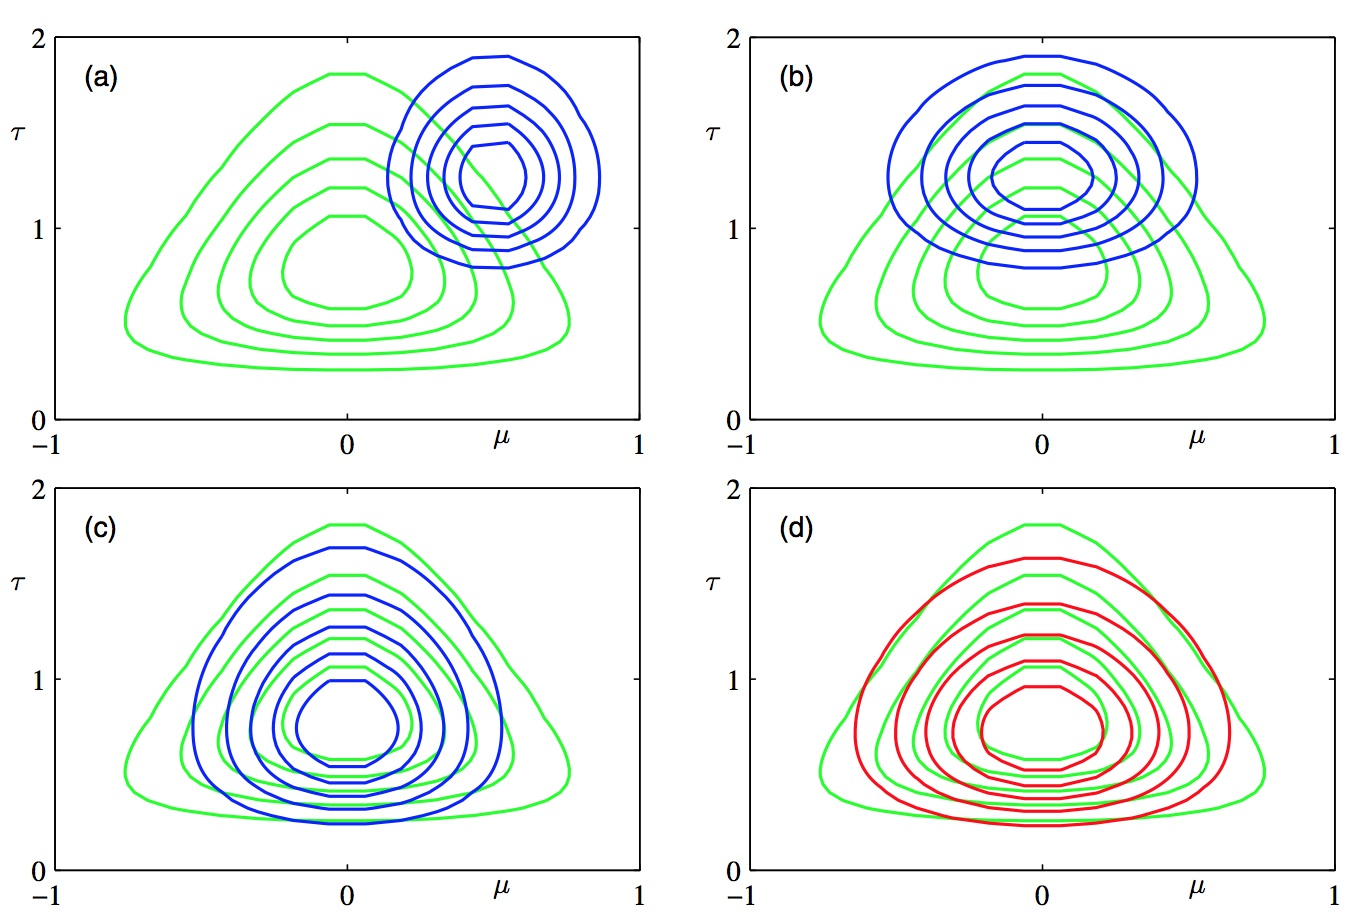
\includegraphics[scale=0.5]{vb_normal_gamma.jpg}
\caption{update for Normal Gamma: figure from \cite{bishop2006pattern}}
     \end{center}
\end{figure}


\subsubsection{update for $q_\mu(\mu)$ and $q_\tau(\tau)$}

In summary, the update for $q_\mu(\mu)$ and $q_\tau(\tau)$ are:

\begin{equation}\begin{split}
q_\mu^*(\mu) &= \N\left( \frac{n \bar{x} + \lambda_0 \mu_0}{n + \lambda_0 } , \E_{q_\tau }[ \tau] (n + \lambda_0) \right)\\
q_\tau^*(\tau) &= \text{Gamma}(a_n, b_n)
\end{split}\end{equation}

where:

\begin{equation}\begin{split}
\begin{cases}
a_n &= \frac{n}{2} + a_0 \\
b_n &= b_0 + \frac{1}{2} \left[ (n + \lambda_0) \E_{q_\mu} [\mu^2] - 2 \left(n \bar{x} + \lambda_0 \mu_0 \right)  \E_{q_\mu} [\mu]   + \sum_{i=1}^n (x_i)^2 + \lambda_0 \mu_0^2 \right] \\
\end{cases}
\end{split}\end{equation}

with:

\begin{equation}\begin{split}
\E_{q_\mu} [\mu] &= \frac{n \bar{x} + \lambda_0 \mu_0}{n + \lambda_0} \\
\E_{q_\mu} [\mu^2] &= \text{Var}_{q_\mu}[\mu] + (\E_{q_\mu} [\mu])^2 = \frac{1}{\E_{q_\tau}[\tau](n + \lambda_0)} + \left(\frac{n \bar{x} + \lambda_0 \mu_0}{n + \lambda_0}\right)^2
\end{split}\end{equation}

Note that $\E_{q_\tau}[\tau] = \frac{a_n}{b_n}$ for the Gamma distribution.

a {\bf part of } the Python code is listed for the variational parameters update. Of course, one needs to look at the full code for the complete picture.

\begin{lstlisting}[language=Python]
def update(self):
self.lambda_n = self.lambda0 + self.N
self.mu_n = (self.lambda0 * self.mu0 + self.N * self.x_bar) / self.lambda_n
self.a_n = self.a0 + self.N / 2
E_tau = self.a_n / self.b_n
E_mu2 = 1 / (E_tau * self.lambda_n) + self.mu_n**2
self.b_n = self.b0 + 0.5 * (np.sum(self.data**2) + 
		self.lambda0 * self.mu0**2 + 
		(self.lambda_n * E_mu2) - 
		2 * (self.N * self.x_bar + self.lambda0 * self.mu0) * self.mu_n)
\end{lstlisting}

\subsection{Interactive Python Program for Variational Inference Visualization}

To visualize the variational inference process for the Normal-Gamma distribution, we can create an interactive Python program using matplotlib. This program will show the true joint distribution $p(\mu, \tau)$ and the variational approximations $q(\mu)$ and $q(\tau)$ after each iteration.

Here's the Python code to implement this visualization:





\newpage


\section{Example of Gaussian Mixture Model \optional}

\subsection{The joint density}

\begin{equation}
\begin{split}
p(X, Z, \mu, \Lambda, \pi) &= p(X | Z, \mu, \Lambda, \pi)p(Z| \mu, \Lambda, \pi)p(\mu| \Lambda, \pi)p( \Lambda | \pi) p( \pi)\\
&= p(X | Z, \mu, \Lambda)p(Z| \pi)p(\mu| \Lambda )p( \Lambda ) p( \pi)
\end{split}
\end{equation}

\subsection{Definitions for each probabilities}

\subsubsection{Definition for $p(Z| \pi)$:}

first, is the probability of mixture indices, $Z = \{ z_1, ..., z_N\}$, given weights $\pi$.

\begin{equation}
\begin{split}
p (Z |\pi) &= \prod^N_{i=1} p(z_i|\pi)\\
&= \prod^N_{i=1} \prod^K_{k=1} \pi^{z_{ik}}_k\\
\end{split}
\end{equation}

The reason for which $\left(p(z_i|\pi) = \prod^K_{k=1} \pi^{z_{ik}}_k \right)$, or $\left(p(z|\pi) = \prod^K_{k=1} \pi^{z_{k}}_k\right)$, is because in Bishop, $z$ is not represented in a scalar form, but rather in a vector of dimension $K$, which has a single element $1$, and the rest are all $0$s. For example, instead of using $p(z_i = 2 | \pi = [0.2, 0.3, 0.5]) = 0.3 $, Bishop uses $p(z_i = [0, 1, 0] | \pi = [0.2, 0.3, 0.5]) = 0.3 $. In any case, this refers to the second element of $\pi$. Therefore, a simpler and vocal representation for $p(z|\pi)$ is just the $z^{th}$ value of $\pi$.

\subsubsection{Definition for $p(X| Z, \mu, \Lambda)$:}

\begin{equation}
\begin{split}
p(X| Z, \mu, \Lambda) &= \prod^N_{i=1} p(x_i | z_i, \mu, \Lambda)\\
&\text{In the normal literature, such as Bilmes, it is defined as:}\\
&= \prod^N_{i=1} \mathcal{N}(x_i | \mu_{z_i}, \Lambda_{z_i}^{-1})\\
&\text{However, due to the vector representation of Bishop, the above is defined as:}\\
&= \prod^N_{i=1} \prod^K_{k=1} \mathcal{N}(x_i | \mu_{k}, \Lambda_{k}^{-1})^{z_{ik}}\\
\end{split}
\end{equation}

However, the above two represent the same thing.

\subsubsection{Definition for $p(\pi)$:}

This is just a straight Dirichlet probability:

\begin{equation}
\begin{split}
p(\pi | \alpha_0) &= \mathrm{Dir}(\pi| \alpha_0) \propto C(\alpha_0) \prod_{k=1}^K \pi_k^{\alpha_{0k} - 1}  \\
&\implies \log p(\pi | \alpha_0) \propto (\alpha_0 -1)  \sum_{k=1}^K \log \pi_k\\
\end{split}
\end{equation}

\subsubsection{Definition for $p(\mu| \Lambda )p( \Lambda )$:}

This is almost always a Gaussian-Wishart distribution:

\begin{equation}
\begin{split}
p (\mu, \Lambda) &= p (\mu | \Lambda) p (\Lambda)\\
&= \prod_{k=1}^K \mathcal{N} (\mu_k | m_0, (\beta_0 \Lambda_k)^{-1} ) \mathcal{W} ( \Lambda_k | W_0, v_0)
\end{split}
\end{equation}



\subsection{Begin VB of GMM}

\subsubsection{The expression for $q^*(Z)$:}

\begin{equation}
\begin{split}
    \log q^*(Z) &= \E_{\pi,\mu,\Lambda} \left[ \log p (X,Z, \pi, \mu, \Lambda)  \right] + \C \\
    &= \E_{\pi} \left[ \log p (Z | \pi)  \right]  + \E_{\mu, \Lambda} \left[ \log p (X | Z, \mu, \Lambda)  \right] + \C \\
    &= \E_{\pi} \left[ \log \prod^N_{i=1} \prod^K_{k=1} \pi^{z_{ik}}_k  \right]  + \E_{\mu, \Lambda} \left[ \log  \prod^N_{i=1} \prod^K_{k=1} \mathcal{N}(x_i | \mu_{k}, \Lambda_{k}^{-1})^{z_{ik}}  \right] + \C \\
    &= \E_{\pi} \left[ \sum^N_{i=1} \sum^K_{k=1} \log \pi^{z_{ik}}_k  \right]  + \E_{\mu, \Lambda} \left[  \sum^N_{i=1} \sum^K_{k=1} \log \mathcal{N}(x_i | \mu_{k}, \Lambda_{k}^{-1})^{z_{ik}}  \right] + \C \\
    &\text{given that:}, ( \log a^b = b \log a):\\
    &= \E_{\pi} \left[ \sum^N_{i=1} \sum^K_{k=1} z_{ik} \log \pi_k  \right]  + \E_{\mu, \Lambda} \left[  \sum^N_{i=1} \sum^K_{k=1} z_{ik} \log \mathcal{N}(x_i | \mu_{k}, \Lambda_{k}^{-1})  \right] + \C \\
    &= \sum^N_{i=1} \sum^K_{k=1} z_{ik} \E_{\pi}  [ \log \pi_k ]  +  \sum^N_{i=1} \sum^K_{k=1} z_{ik} \E_{\mu, \Lambda} [ \log \mathcal{N}(x_i | \mu_{k}, \Lambda_{k}^{-1}) ]  + \C \\
    &\text{Taking the common term to the left}, \sum^N_{i=1} \sum^K_{k=1} z_{ik}:\\
    &= \sum^N_{i=1} \sum^K_{k=1} z_{ik} \left( \E_{\pi}  [ \log \pi_k ]  + \E_{\mu, \Lambda} [ \log \mathcal{N}(x_i | \mu_{k}, \Lambda_{k}^{-1}) ] \right) + \C \\
    &\text{Bishop nominates a new term:} \log \rho_{ik} \\
    &= \sum^N_{i=1} \sum^K_{k=1} z_{ik} \left( \log \rho_{ik} \right) + \C \\
\end{split}
\end{equation}

Let's look at the expression for $\log \rho_{ik}$:

\begin{equation}
\begin{split}
    \log \rho_{ik} &= \E_{\pi}  [ \log \pi_k ]  + \E_{\mu_k, \Lambda_k} [ \log \mathcal{N}(x_i | \mu_{k}, \Lambda_{k}^{-1})] \\
    &= \E_{\pi}  [ \log \pi_k ]  + \E_{\mu_k, \Lambda_k} \left[ \log \left( \frac{1}{(2\pi)^{(d/2)} } | \Lambda_k |^{1/2} \exp \left( -\frac{1}{2} (x_i - \mu_{k})^\top \Lambda_k (x_i - \mu_{k}) \right) \right) \right] \\
    &= \E_{\pi}  [ \log \pi_k ]  + \E_{\mu_k, \Lambda_k} \left[ \log (2\pi)^{\frac{-d}{2}} + \frac{1}{2} \log |\Lambda_k| + \left( -\frac{1}{2} (x_i - \mu_{k})^\top \Lambda_k (x_i - \mu_{k}) \right) \right] \\
    &= \E_{\pi}  [ \log \pi_k ]  + \E_{\mu_k, \Lambda_k} \left[ \frac{-d}{2} \log (2\pi) + \frac{1}{2} \log |\Lambda_k| - \left( \frac{1}{2} (x_i - \mu_{k})^\top \Lambda_k (x_i - \mu_{k}) \right) \right] \\
    &= \E_{\pi}  [ \log \pi_k ]  + \frac{-d}{2} \log (2\pi) + \frac{1}{2} \E_{\Lambda_k} \left[  \log |\Lambda_k| \right] - \frac{1}{2} \E_{\mu_k, \Lambda_k} \left[   (x_i - \mu_{k})^\top \Lambda_k (x_i - \mu_{k})  \right] \\
\end{split}
\end{equation}

Now, with $\log q^*(Z)$ expressed in terms of $\log \rho_{ik}$:

\begin{equation}
\begin{split}
    \log q^*(Z) &= \sum^N_{i=1} \sum^K_{k=1} z_{ik} \left( \log \rho_{ik} \right) + \C \implies\\
   q^*(Z) &= \exp \left( \sum^N_{i=1} \sum^K_{k=1} z_{ik} \left( \log \rho_{ik} \right) + \C \right)\\
    &=  C \prod^N_{i=1} \prod^K_{k=1} \exp ( z_{ik} \left( \log \rho_{ik} )  \right)
    =  C \prod^N_{i=1} \prod^K_{k=1} \exp \left( \log \rho_{ik}^{z_{ik}} \right) 
   =  C \prod^N_{i=1} \prod^K_{k=1} \rho_{ik}^{z_{ik}} \\
\end{split}
\end{equation}

Since  $q^*(Z) = \prod^N_{i=1}q^*(z_i)$:

\begin{equation}
\begin{split}
  q^*(Z) &=  \prod^N_{i=1} C \prod^K_{k=1} \rho_{ik}^{z_{ik}} \\
\end{split}
\end{equation}

In a way,  $\rho_{ik}^{z_{ik}}$ plays the same role as  $\pi \text{ in } p(z_i|\pi)$, therefore, just as $\sum^K_{k=1} \pi_k = 1$, we need to normalize $\rho_{ik}$ over $k$:

\begin{equation}
\begin{split}
    q^*(Z) &= \prod_{i=1}^N q^*(z_i) =  \prod^N_{i=1} \left(\frac{1}{ \sum^K_{j=1} \rho_{ij}} \prod^K_{k=1} \rho_{ik}^{z_{ik}} \right) \\
    &=  \prod^N_{i=1} \prod^K_{k=1} \frac{\rho_{ik}^{z_{ik}}}{ \sum^K_{j=1} \rho_{ij}}
    =  \prod^N_{i=1} \prod^K_{k=1} r_{ik}^{z_{ik}}\\
\end{split}
\end{equation}

This is a multinomial distribution, therefore, $\E [z_{ik} ] = r_{ik}$

\subsubsection{The expression for $q^*(\pi,\mu,\Lambda)$:}

\begin{equation}
\begin{split}
    \log q^*(\pi,\mu,\Lambda) &= \E_{Z} \left[ \log p (X,Z, \pi, \mu, \Lambda)  \right] + \C \\
    &= \E_{Z} \left[ \log p (X | Z, \mu, \Lambda)  \right] + \E_{Z} \left[ \log p ( Z | \pi)  \right] + \E_{Z} \left[ \log p (\pi)  \right] +\E_{Z} \left[ \log p ( \mu | \Lambda)  \right] + \E_{Z} \left[ \log p (\Lambda)  \right] + \C \\
    &= \E_{Z} \left[ \log p (X | Z, \mu, \Lambda)  \right] + \E_{Z} \left[ \log p ( Z | \pi)  \right] + \log p (\pi) + \log p ( \mu | \Lambda) + \log p (\Lambda) + \C \\
\end{split}
\end{equation}

Combine the mean and precision together:

\begin{equation}
\begin{split}
    &= \E_{Z} \left[ \log p (X | Z, \mu, \Lambda)  \right] + \E_{Z} \left[ \log p ( Z | \pi)  \right] + \log p (\pi) + \log p ( \mu, \Lambda) + \C \\
    &\text{And since each }  ( \mu_k, \Lambda_k) \text{ is independent, therefore:} \\
    &= \E_{Z} \left[ \log  \prod^N_{i=1} \prod^K_{k=1} \mathcal{N}(x_i | \mu_{k}, \Lambda_{k}^{-1})^{z_{ik}}  \right] + \E_{Z} \left[ \log p ( Z | \pi)  \right] + \log p (\pi) + \sum^K_{k=1} \log p ( \mu_k, \Lambda_k) + \C \\
    &= \E_{Z} \left[  \sum^N_{i=1} \sum^K_{k=1} z_{ik} \log \mathcal{N}(x_i | \mu_{k}, \Lambda_{k}^{-1})  \right] + \E_{Z} \left[ \log p ( Z | \pi)  \right] + \log p (\pi) + \sum^K_{k=1} \log p ( \mu_k, \Lambda_k) + \C\\
     &=  \sum^K_{k=1} \sum^N_{i=1} \E_{Z}[ z_{ik}] \log \mathcal{N}(x_i | \mu_{k}, \Lambda_{k}^{-1})  + \E_{Z} \left[ \log p ( Z | \pi)  \right] + \log p (\pi) + \sum^K_{k=1} \log p ( \mu_k, \Lambda_k) + \C\\
     &= \underbrace{ \E_{Z} \left[ \log p ( Z | \pi)  \right] + \log p (\pi)}_{\log q^*(\pi)} + \underbrace{ \sum^K_{k=1} \sum^N_{i=1} \E_{Z}[ z_{ik}] \log \mathcal{N}(x_i | \mu_{k}, \Lambda_{k}^{-1})  +  \sum^K_{k=1} \log p ( \mu_k, \Lambda_k)}_{\log q^*(\mu,\Lambda)} + \C\\
\end{split}
\end{equation}

For the part of $\log q^*(\pi)$:

\begin{equation}
\begin{split}
\log q^*(\pi) &= \E_{Z} \left[ \log p ( Z | \pi)  \right] + \log p (\pi)\\
&= \E_{Z} \left[  \log \prod^N_{i=1} \prod^K_{k=1} \pi^{z_{ik}}_k \right] + \log p (\pi)\\
&= \E_{Z} \left[   \sum^N_{i=1} \sum^K_{k=1} z_{ik} \log \pi_k \right] + \log p (\pi)\\
&=  \sum^N_{i=1} \sum^K_{k=1} \log \pi_k  \E_{Z} [z_{ik}] + (\alpha_0 -1)  \sum_{k=1}^K \log \pi_k + \C \\
&=  \sum^K_{k=1} \log \pi_k   \sum_{i=1}^N r_{i,k} + (\alpha_0 -1)  \sum_{k=1}^K \log \pi_k + \C \\
&=  \sum^K_{k=1} \Bigg( \underbrace{ \sum_{i=1}^N r_{i,k} + \alpha_0}_{a_k} -1 \Bigg) \log \pi_k  + \C
\implies q^*(\pi) = \text{Dir} \left( \pi | a_1, \dots, a_K \right)
\end{split}
\end{equation}



For the part of $\log q^*(\mu,\Lambda)$:

\begin{equation}
\begin{split}
\log q^*(\mu,\Lambda) &= \sum^K_{k=1} \sum^N_{i=1} \E_{Z}[ z_{ik}] \log \mathcal{N}(x_i | \mu_{k}, \Lambda_{k}^{-1})  +  \sum^K_{k=1} \log p ( \mu_k, \Lambda_k)\\
&\text{We have the expression for $\E_{q^*(Z)}[Z]$ from the previous section, i.e., $\E_{q^*(Z)}[z_{ik}] = r_{ik}$}:
\end{split}
\end{equation}

\begin{figure}[H]
    \begin{center}
    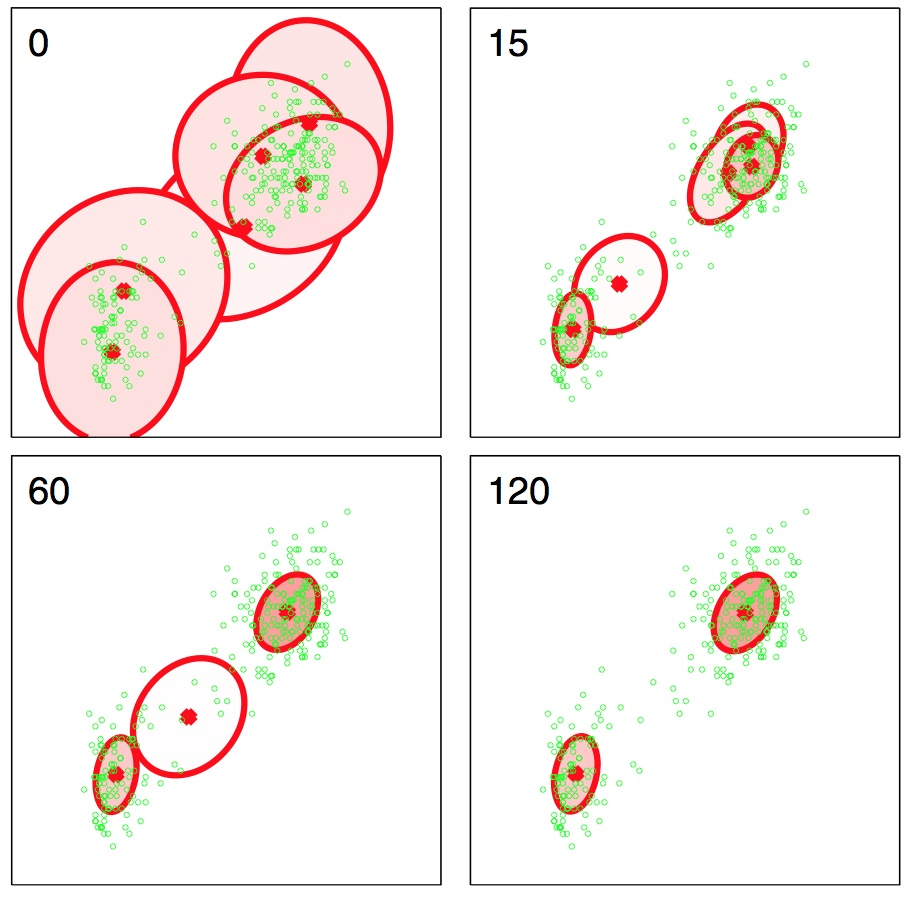
\includegraphics[scale=0.5]{vb_gmm.jpg}
\caption{update for Gaussian Mixture Model: figure from \cite{bishop2006pattern}}
     \end{center}
\end{figure}

\newpage


%\subsection{Log-likelihood and Evidence Lower Bound (ELOB)}
%\begin{itemize}
%\item 
%It is universally true that: 
%\begin{equation}\nonumber
% \log{(p(\x))} =  \log{ (p(\x,\z)) } - \log{ (p(\z|\x)) }
%\end{equation}
%
%\item
%It's also true (a bit silly) that:
%
%\begin{equation}\nonumber
%    \log{(p(\x))} =  [ \log (p(\x,\z))  - \log(q(Z)) ] - [ \log (p(\z|\x)) - \log (q(Z))]       
%\end{equation}
%
%\item 
%The above is so that we can insert an arbitrary pdf $q(Z)$ into, now we get:
%
%\begin{equation}
%    \log{(p(\x))} =   \log{  \left(   \frac{p(\x,\z)}{q(Z)}  \right)  } - 
%                    \log{  \left(   \frac{p(\z|\x)}{q(Z)}  \right)  }     \nonumber
%\end{equation}
%
%\item
%Taking the expectation on both sides, given $q(Z)$:
%
%
%\begin{equation}\nonumber
%\begin{split}
%    \log{(p(\x))} &=  \int q(Z) \log{  \left(   \frac{p(\x,\z)}{q(Z)}  \right)  } \d \z - \int q(Z) \log{  \left(   \frac{p(\z|\x)}{q(Z)}  \right)  } \d \z\\
%&=  \underbrace{\int q(Z) \log  ( p(\x,\z) )  \d \z - \int q(Z) \log (  q(Z) ) \d \z}_{\text{ELBO}(q)} + \underbrace{\left( - \int q(Z) \log{  \left(   \frac{p(\z|\x)}{q(Z)}  \right)  } \d \z \right)}_{\KL(q\|p)}\\  
%&=  \text{ELBO}(q) + \KL(q\|p)\\
%\end{split}
%\end{equation}
%
%\end{itemize}
%
%
%%-------------------------------------------------------------
%
%\subsection{Alternative Evidence Lower Bound (ELOB)}
%
%We often see the following alternative derivation:
%
%\begin{equation}\nonumber
%\begin{split}
%    \log{(p(\x))} &=  \log \int_Z p(\x,\z) \d \z\\
%&=  \log \int_Z p(\x,\z) \frac{q(Z)}{q(Z)} \d \z\\
%&=  \log \left( \E_{q} \left[ \frac{p(\x,\z)}{q(Z)} \right] \right)\\
%&\geq    \E_{q} \left[\log   \left(\frac{p(\x,\z)}{q(Z)}  \right) \right] \text{using Jensen's inequality} \\
%&=   \E_{q} \left[\log  ( p(\x,\z) ) \right] - \E_{q} \left[ \log (q(Z)) \right]  \\
%& \triangleq  \text{ELBO}(q) \\
%\end{split}
%\end{equation}
%
%It can be proven easily that the ``missing'' part, i.e., $\log{(p(\x))} - \text{ELBO}(q) = \KL(q\|p)$.
%
%
%
%
%%-------------------------------------------------------------
%
%\subsection{Maximize Evidence Lower Bound (ELOB)}
%
% 
%
%\begin{equation}\nonumber
%\begin{split}
%    \log{(p(\x))} =  \text{ELBO}(q) + \KL(q\|p)\\
%\end{split}
%\end{equation}
%
%\begin{itemize}
%
%\item 	We can give a name to both terms:
%
%\begin{equation}\nonumber
%\begin{split}
%\text{Evidence Lower Bound (ELOB):}\hspace{10 mm}& \text{ELBO}(q) = \int q(Z) \log  ( p(\x,\z) )  \d \z - \int q(Z) \log (  q(Z) ) \d \z\\
%\text{KL divergence:} \hspace{10 mm}& \KL(q\|p) = \int q(Z) \log{  \left(   \frac{p(\z|\x)}{q(Z)}  \right)  } \d \z \\
%\end{split}
%\end{equation}
%
%
%
%\item Notice $p(\x)$ is fixed with respect to the choice of $q(Z)$. We wanted to choose a $q(Z)$ function that minimize KL divergence, so that $q(Z)$ becomes closer and closer to $p(\z|\x)$. Of course, let's see what happens when $q(Z) = p(\z|\x)$:
%
%\begin{equation}
% \KL(q\|p) = - \int p(\z|\x) \log{  \left(   \frac{p(\z|\x)}{p(\z|\x)}  \right)  } \d \z = 0 \nonumber
%\end{equation}
%
%\item We know that $p(\x) = \text{ELBO}(q) + \KL(q\|p) $. Minimizing $\KL (q\| p)$ is the same as maximizing the Evidence Lower Bound $\text{ELBO}(q)$.
%
%\end{itemize}
%
%
%
%
%
%
%%-------------------------------------------------------------
%
%\subsection{Approach One}
%
%\begin{itemize}
%
%\item Arbitrary (i.e., non Exponential Family ) distributions
%
%\item No maximizing variational distribution parameters
%
%\end{itemize}
%
%
%
%%-------------------------------------------------------------
%
%\subsection{The choice of $q(Z)$}
%
%
%\begin{itemize}
%
%\item
%Suppose let's choose $q(Z)$, such that:
%
%\begin{equation}\nonumber
% q(Z) = \prod_{i=1}^M q_i(z_i)
%\end{equation}
%
%\item
%Substitute this choice into Evidence Lower Bound (ELOB):
%
%\begin{equation}\nonumber
% \begin{split}
%\text{ELBO}(q) &= \int q(Z) \log  ( p(\x,\z) )  \d \z - \int q(Z) \log (  q(Z) ) \d \z\\
% &= \underbrace{ \int \prod_{i=1}^M q_i(z_i)\log{(p(\x,\z))} \d \z}_{\text{part (1)}} - \underbrace{\int \prod_{i=1}^M q_i(z_i)\sum_{i=1}^M \log { (q_i(z_i))}\d \z}_{\text{part (2)}}\\
% \end{split}
%\end{equation}
%
%\end{itemize}
%
%
%
%%-------------------------------------------------------------
%
%\subsection{Simplification of (Part 1):}
%
% 
%
%\begin{equation}\nonumber
% \begin{split}
% &\text{(Part 1)} = \int \prod_{i=1}^M q_i(z_i) \log{(p(\x,\z))} \d \z\\
% &\int\limits_{Z_1} \int\limits_{Z_2}... \int\limits_{Z_M}  \prod_{i=1}^M q_i(z_i)  \log{(p(\x,\z))} \d \z_1, \d \z_2, \dots, \d \z_M
% \end{split}
%\end{equation}
%
%
%\begin{itemize}
%
%\item
%Rearrange the expression by taking a particular $q_j(z_j)$ out of the integral:
%
%
%\begin{equation}
% \text{(Part 1)} = \int\limits_{z_j} q_j(z_j) \left(  \idotsint\limits_{Z_{i \neq j}} \prod_{ i \neq j}^M q_i(z_i) \log{(p(\x,\z))} \prod_{ i \neq j}^M \d z_i \right)  \d z_j
% \nonumber
%\end{equation}
%
%\item
%or, more compactly:
%
%\begin{equation}
% \text{(Part 1)} = \int\limits_{z_j} q_j(z_j) \left(  \idotsint\limits_{Z_{i \neq j}}  \log{(p(\x,\z))} \prod_{ i \neq j}^M q_i(z_i)\d z_i  \right)  \d z_j
% \nonumber
%\end{equation}
%
%\item or, even more meaningfully, it can be put into an expectation function, and since $\prod_{ i \neq j}^M q_i(z_i)$ is a joint probability density
%
%\begin{equation}\nonumber
% \text{(Part 1)} = \int\limits_{z_j} q_j(z_j) \left[  \E_{i\neq j} \bigg[ \log{(p(\x,\z))} \bigg]   \right]  \d z_j
%\end{equation}
%
%\end{itemize}
%
%
%
%
%
%%-------------------------------------------------------------
%
%\subsection{Simplification of (Part 2):}
%
% 
%
%\begin{equation}\nonumber
% \text{(Part 2)} = \int \prod_{i=1}^M q_i(z_i)\sum_{i=1}^M \log { (q_i(z_i))}\d \z
% \nonumber
%\end{equation}
%
%
%\begin{itemize}
%
%\item
%
%Note that the above needs to integrate out all $Z = \{z_1, ..., z_M \}$, which is quite daunting. However, notice that each term in the sum, $\sum_{i=1}^M \log { (q_i(z_i))}$ involves only a single $i$, therefore, we are able to simplify the above into the following:
%
%\begin{equation}
% \text{(Part 2)} = \sum_{i=1}^M \left( \int\limits_{z_i} q_i(z_i)  \log { (q_i(z_i))} \d z_i \right)
% \nonumber
%\end{equation}
%
%\item
%For a particular $p_j(z_j)$, the rest of the sum can be treated like a constant, part 2 can be written as:
%
%\begin{equation}
% \text{(Part 2)} = \int\limits_{z_j} q_i(z_i) \log { (q_i(z_i))} \d z_j + \C
% \nonumber
%\end{equation}
%
%\hspace{5 mm} where $\C$ are the term does not involve $z_j$.
%\end{itemize}
%
%
%
%
%
%
%%-------------------------------------------------------------
%
%\subsection{Putting Part (1) and Part (2) together:}
%
% 
%
%\begin{equation} \nonumber
% \begin{split}
% \text{ELBO}(q) &= \text{Part (1)} - \text{Part (2)}
%= \int\limits_{z_j} q_j(z_j)  \E_{i\neq j} \bigg[ \log{(p(\x,\z))} \bigg]  \d z_j - \int\limits_{z_j} q_j(z_j) \log { (q_j(z_j))} \d z_j + \C\\
% \end{split}
%\end{equation}
%
%
%\begin{itemize}
%
%\item
%
%Note that  $\E_{i\neq j} \left[ \log{(p(\x,\z))} \right]$ would be some $\log [p (z_i)]$, we name it $ \log( \tilde{p_j} (X, z_j)) $, i.e.,:
%
%\begin{equation} \nonumber
% \begin{split}
% \log( \tilde{p_j} (X, z_j)) = \E_{i\neq j} \left[ \log{(p(\x,\z))} \right]
%\end{split}
%\end{equation}
%
%\item
%Or equivalently we can express Evidence Lower Bound (ELOB) in terms of:
%
%\begin{equation}
% \L(q_j) = \int\limits_{z_j} q_j(z_j) \log \left[  \frac{\tilde{p_j}(X,z_j)} { q_j(z_j) }   \right] + \C.
% \nonumber
%\end{equation}
%
%This is the same as $- \KL \bigg( \E_{i\neq j} \left[ \log{(p(\x,\z))} \right] \|  q_i(z_i) \bigg) $
%
%\item
%{\bf This is the key}: We can maximize ELOB, or $\text{ELBO}(q)$, by minimizing this special KL divergence, where we can find approximate and optimal  $q_{i}^*(z_i)$, such that:
%
%\begin{equation} \nonumber
%    \log{ ( q_{i}^*(z_i)) } = \E_{i\neq j} \big[ \log{(p(\x,\z))} \big]
%\end{equation}
%\end{itemize}
%
%
%
%
%
%-------------------------------------------------------------

%\subsection{Example: Gaussian-Gamma Conjugate prior}
%
%\begin{itemize}
%
%\item Let $\mathcal{D} = \{x_1, \dots x_n \}$:
%
%\begin{equation}\nonumber
%\begin{split}
%p ( \mathcal{D}| \mu, \tau ) &= \prod_{i=1}^n \left( \frac{\tau}{2 \pi}  \right)^{\frac{1}{2}}   \exp \left( \frac{-\tau}{2} (x_i - \mu)^2 \right) \\
% &=  \left( \frac{\tau}{2 \pi} \right)^{\frac{n}{2}}   \exp \left( \frac{-\tau}{2} \sum_{i=1}^n (x_i - \mu)^2 \right) \\
%\end{split}
%\end{equation}
%
%\begin{equation}\nonumber
%\begin{split}
%p ( \mu | \tau ) &= \mathcal{N} (\mu_0,  (\lambda_0 \tau)^{-1}) \propto \exp \left( \frac{-\lambda_0 \tau}{2} (\mu - \mu_0)^2 \right) \\
%p(\tau) &=  \text{Gamma}( \tau | a_0, b_0) \propto \tau^{a_0-1}\exp^{-b_0 \tau} \\
%\end{split}
%\end{equation}
%
%\item Complete data-likelihood is:
%
%\end{itemize}
%
%\begin{equation}\nonumber
%\begin{split}
%p ( \mathcal{D},  \mu, \tau ) = p ( \mathcal{D}| \mu, \tau ) p ( \mu | \tau ) p(\tau)\\
%\end{split}
%\end{equation}
%
%
%
%%-------------------------------------------------------------
%
%\subsection{Of course, due to conjugacy, the solution can be found exactly:}
%
%
%\begin{equation}\nonumber
%\begin{split}
%p (  \mu,  \tau | \D ) &\propto p ( \mathcal{D}| \mu, \tau )  p (\mu | \tau) p(\tau) =  \mathcal{N} (\mu_n,  (\lambda_n \tau)^{-1})\text{Gamma}( \tau | a_n, b_n) \\
%\end{split}
%\end{equation}
%
%\hspace{15 mm} where:
%
%\begin{equation}\nonumber
%\begin{split}
%\mu_n & =\frac{\lambda_0 \mu_0 + n \bar{x}}{\lambda_0 + n}\\
%\lambda_n &= \lambda_0 + n\\
%a_n &= a_0 + n/2 \\
%b_n &= b_0 + \frac{1}{2} \sum_{i=1}^n (x_i - \bar{x})^2 +  \frac{\lambda_0 n (\bar{x} - \mu_0)^2}{2(\lambda_0 + n)}\\
%\end{split}
%\end{equation}
%
%
%However, for demo purpose, we assume $q (\mu, \tau) $:
%
%\begin{equation}\nonumber
%\begin{split}
%q (\mu, \tau) &= q_{\mu} (\mu) q_{\tau}(\tau)\\
%\end{split}
%\end{equation}
%
%
%
%%-------------------------------------------------------------
%
%\subsection{Computing $\log{ ( q_\mu^*(\mu)) } = \E_{q_\tau(\tau)}  \left[ \log{(p(\mu, \tau | \mathcal{D}))} \right]$ (1) }
%
% 
%
%\begin{equation}\nonumber
%\begin{split}
%    \log{ ( q_\mu^*(\mu)) } &= \E_{q_\tau}  \left[ \log{(p(\mu, \tau | \mathcal{D}))} \right]\\
%&= \E_{q_\tau}  \left[ \log ( p ( \mathcal{D}| \mu, \tau ) ) +  \log p (\mu | \tau) \right] + \C \hspace{5 mm} \text{ remove terms do NOT contain } \mu \\
%&= \E_{q_\tau}  \left[ \underbrace{  - \frac{\tau}{2} \sum_{i=1}^n (x_i - \mu)^2 }_{\log ( p ( \mathcal{D}| \mu, \tau ) )} \underbrace{ +  \frac{\lambda_0 \tau}{2} (\mu - \mu_0)^2}_{\log p (\mu | \gamma) }    \right] + \C \\
%&= -  \frac{\E_{q_\tau }[ \tau] }{2}    \underbrace{\left[  \sum_{i=1}^n (x_i - \mu)^2  +  \lambda_0 (\mu - \mu_0)^2  \right]}_{\text{terms contain } \mu \text{ but does not contain } \tau} + \C \\
%\end{split}
%\end{equation}
%
%Completing the square for the $\mu$ terms:
%
%
%\begin{equation}\nonumber
%\begin{split}
%&\sum_{i=1}^n (x_i - \mu)^2  +  \lambda_0 (\mu - \mu_0)^2 = n \mu^2 - 2 n \mu \bar{x}  + \lambda_0 \mu^2 - 2 \lambda_0 \mu_0 \mu + \C \\
%%--------------------------
%= & (n + \lambda_0) \mu^2 - 2 \mu (n \bar{x} + \lambda_0 \mu_0 ) 
%%---------------------------
%=(n + \lambda_0) \left( \mu^2 - \frac{  2 \mu (n \bar{x} + \lambda_0 \mu_0)}{(n + \lambda_0) }  \right) \\
%%--------------------------
%=&(n + \lambda_0) \left( \mu - \frac{(n \bar{x} + \lambda_0 \mu_0)}{(n + \lambda_0) }  \right)^2 + \C \\
%%--------------------------
%\end{split}
%\end{equation}
%
%
%
%
%
%
%%-------------------------------------------------------------
%
%\subsection{Computing $\log{ ( q_\mu^*(\mu)) } = \E_{q_\tau(\tau)}  \left[ \log{(p(\mu, \tau | \mathcal{D}))} \right]$ (2) }
%
% 
%
%Therefore, we have:
%
%\begin{equation}\nonumber
%\begin{split}
%    \log{ ( q_\mu^*(\mu)) } &= -  \frac{\E_{q_\tau }[ \tau] }{2}    \left[  \sum_{i=1}^n (x_i - \mu)^2  +  \lambda_0 (\mu - \mu_0)^2  \right] + \C \\
%&= -  \frac{\E_{q_\tau }[ \tau] (n + \lambda_0) }{2}    \left( \mu - \frac{(n \bar{x} + \lambda_0 \mu_0)}{(n + \lambda_0) }  \right)^2 + \C \\
%&= \N\left( \frac{n \bar{x} + \lambda_0 \mu_0}{n + \lambda_0 } , \E_{q_\tau }[ \tau] (n + \lambda_0) \right)
%\end{split}
%\end{equation}
%
%
%
%
%
%
%
%%-------------------------------------------------------------
%
%\subsection{Computing $\log{ ( q_{i}^*(\tau)) } = \E_{q_\mu(\mu)}  \left[ \log{(p(\mu, \tau | \mathcal{D}))} \right]$ (1)}
%
% 
%
%\begin{equation}\nonumber
%\begin{split}
%    \log{ ( q_\tau^*(\tau)) } &= \E_{q_\mu}  \left[ \log{(p(\mu, \tau | \mathcal{D}))} \right]\\
%&= \E_{q_\mu}  \left[ \log ( p ( \mathcal{D}| \mu, \tau ) ) +  \log p (\mu | \tau) + \log p ( \tau)   \right] + \C \\
%&= \E_{q_\mu}  \left[ \underbrace{ \frac{n}{2 }  \log \left( \tau \right) - \frac{\tau}{2} \sum_{i=1}^n (x_i - \mu)^2 }_{\log ( p ( \mathcal{D}| \mu, \tau ) )} \underbrace{ -  \frac{\lambda_0 \tau}{2} (\mu - \mu_0)^2}_{\log p (\mu | \gamma) }  \underbrace{+ (a_0-1) \log (  \tau )  -b_0 \tau}_{\log p ( \tau) }   \right] + \C \\
%\end{split}
%\end{equation}
%
%Bring terms without $\mu$ outside of the integral:
%
%\begin{equation}\nonumber
%\begin{split}
%&= \frac{n}{2 }\log ( \tau ) + (a_0-1) \log (  \tau )  -b_0 \tau - \frac{\tau}{2} \E_{q_\mu(\mu)}  \left[   \sum_{i=1}^n (x_i - \mu)^2  +  \lambda_0(\mu - \mu_0)^2 \right] + \C \\
%&= \left(  \underbrace{ \frac{n}{2 } + a_0   }_{a_n}  -1 \right) \log ( \tau )  - \tau \left( \underbrace{ b_0  + \frac{1}{2} \E_{q_\mu(\mu)}  \left[   \sum_{i=1}^n (x_i - \mu)^2  +  \lambda_0(\mu - \mu_0)^2 \right] }_{b_n} \right)+ \C \\
%\end{split}
%\end{equation}
%
%
%
%
%
%%-------------------------------------------------------------
%
%\subsection{Computing $\log{ ( q_{i}^*(\tau)) } = \E_{q_\mu(\mu)}  \left[ \log{(p(\mu, \tau | \mathcal{D}))} \right]$ (2)}
%
% 
%
%We can rewrite,
%
%\begin{equation}\nonumber
%\begin{split}
%b_n &= b_0 + \frac{1}{2} \E_{q_\mu}  \left[   \sum_{i=1}^n (x_i - \mu)^2  +  \lambda_0(\mu - \mu_0)^2 \right] \\
%%------------------
%&= b_0 + \frac{1}{2} \E_{q_\mu}  \left[  - 2 \mu n \bar{x}  + n \mu^2 +  \lambda_0 \mu^2 - 2 \lambda_0 \mu_0 \mu \right] + \sum_{i=1}^n (x_i)^2 + \lambda_0 \mu_0^2 \\
%&=  b_0 + \frac{1}{2} \left[ (n + \lambda_0) \E_{q_\mu} [\mu^2] - 2 \left(n \bar{x} + \lambda_0 \mu_0 \right)  \E_{q_\mu} [\mu]   + \sum_{i=1}^n (x_i)^2 + \lambda_0 \mu_0^2 \right] \\
%\end{split}
%\end{equation}
%
%We will compute $\E_{q_\mu} [\mu]$ and $\E_{q_\mu} [\mu^2]$ since we know of $q_\mu(\mu)$ from previously.
%
%
%
%
%
%%-------------------------------------------------------------
%
%\subsection{Figure and Demo}
%
%\begin{figure}
%    \begin{center}
%    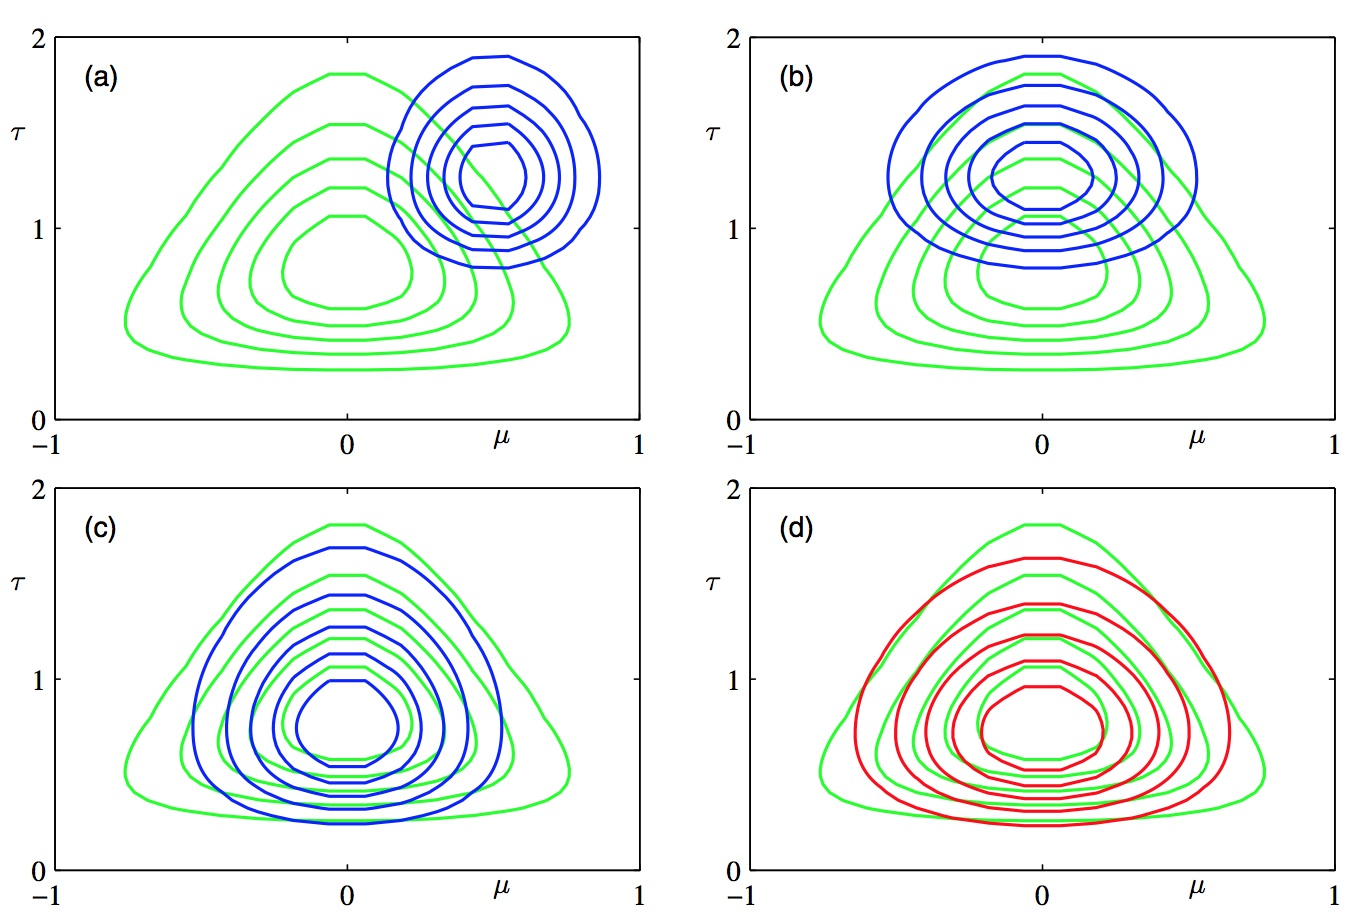
\includegraphics[scale=0.4]{vb_normal_gamma.jpg}
%     \end{center}
%\end{figure}
%
%Also see Matlab Demo!


%
%
%%------------------------------------------------------------------------
%
%\subsection{Approach Two}
%
%\begin{itemize}
%\item Perform direct maximisation over $q(Z)$ using variational calculus
%\end{itemize}
%
%
%
%
%%------------------------------------------------------------------------
%
%\subsection{Functional identity}
%
%\begin{equation}\nonumber
%\begin{split}
% G(f_x(x), f_y(y)) &= \int_x \int_y f_x(x) f_y(y) \log p(x,y) \D x \D y  \implies \\
%%------------------
% \frac{ \delta G(f_x(x), f_y(y)) }{ \delta f_x(x')} &= \int_x \int_y \frac{\delta f_x(x)}{\delta f_x(x')} f_y(y) \log p(x,y) \D x \D y\\
%%------------------
%&= \int_x \int_y  \delta(x - x')  f_y(y) \log p(x,y) \D x \D y\\
%&= \int_y   f_y(y) \log p(x',y)  \D y\\
%\end{split}
%\end{equation}
%
%Let $Z \triangleq (z, \theta)$ \hspace{5 mm} $p(X, Z, \theta) = p(X, Z | \theta) p (\theta)$ \hspace{5 mm} $q(Z, \theta) = \qZ \qtheta$:
%
%Evidence Lower Bound (ELBO) can be written as:
%




%------------------------------------------------------------------------

\section{Variational update in Exponential Family distribution}
%
%\begin{itemize}
%\item Exponential Family distributions
%\item Maximizing variational distribution parameters
%\item Introduction to Stochastic Variational Inference (SVI)
%\end{itemize}

\subsection{Big picture}

Given both the prior and likelihood are exponential family distributions and they form a conjugate pair, then the variational inference (also mean-field approximation), i.e., $q(\z) = \prod_i q_i(z_i)$ can have the following update formula:

\begin{equation}\begin{split}\label{eq exponential family update}
\eta_j =  \E_{q(\z \setminus z_j | \cdot)} [\eta_\post (\z \setminus z_j )]
\end{split}\end{equation}

where $\eta_\post (\z \setminus z_j )$ is the natural parameter associated with posterior distribution $p( z_j \; | \; \z \setminus z_j , \x  )$, i.e., we can express it as: 

\begin{equation}
	\begin{split}
	p_{\eta_\post (\z \setminus z_j )}( z_j \; | \; \z \setminus z_j , \x  )
	\end{split}
\end{equation}

I know the probability form of the above seems to be very complicated, however, you will see that it is no different from how we normally express distributions, $p_{\theta}(\z | \x)$, where:


\begin{equation}\begin{split}
p_{\underbrace{\theta}_{\text{parameters}}}(\underbrace{\z}_{\text{variable}} | \underbrace{\x}_{\text{ conditioning variables}})
\end{split}\end{equation}


\vspace{2mm}

It is very important to note that we are expressing a posterior distribution $p(\cdot) $ in terms of variable $z_j$. Therefore the variables $\z \setminus z_j$ are now part of the parameters of the distribution, hence we use $\eta_\post (\z \setminus z_j )$ to denote the natural parameter of the distribution $p(z_j | -)$.


This can be made much clearer by using an example: if we have a posterior distribution concerning $z_1, \dots, z_3$, and we are interested in the posterior distribution of $z_2$ given $z_1$ and $z_3$ and $\x$, i.e.,


\begin{equation}\begin{split}
p(z_2 \; | \; \z \setminus z_2 , \x )
&= p(z_2 \; | \; z_1, z_3, \x )\\
&\equiv p_{\eta_\post (z_1, z_3 )}(z_2 \; | \; z_1, z_3, \x )
\end{split}\end{equation}

then the update formula for $q_{\eta_2}(z_2)$ is:

\begin{equation}\begin{split}
\eta_2 =  \E_{q(z_1, z_3)} \big[ \eta_\post (z_1, z_3 ) \big]
\end{split}\end{equation}

\vspace{2mm}
compare this with the generic update formula:

\begin{equation}\begin{split}
\log{ ( q_{j}^*(z_j)) } &= \E_{\z \setminus z_j} \big[ \log{(p(\x,\z))} \big]
\end{split}\end{equation}

using exponential family update formula Eq.(\ref{eq exponential family update}), the update is directly applied to the parameter. 

\subsubsection{where is the catch?}

Sounds too easy? Yes, it is! However, it is important to note that this is only applicable to exponential family distributions and conjugacy, and also $\eta$ is the natural parameter when we are dealing with exponential family distributions. Then, obviously, we need to study a few things:

\begin{enumerate}
\item What is an exponential family distribution?
\item What is a natural parameter?
\item What is conjugacy?
\end{enumerate}

Let's talk about exponential family distribution first.

%-------------------------------------------------------------
\subsection{What is Exponential Family?}



Most of the distributions we are going to look at are from the {\bf exponential family}. They are expressed in terms of their natural parameter $\eta$:

\begin{equation}\begin{split}\label{eq exponential family distribution formula}
h(x) \exp \big(   T(x)^\top \eta  - A(\eta)   \big)\\
\end{split}\end{equation}

\begin{equation}\begin{split}
\underbrace{\exp( - A(\eta))}_{\text{normalization}} h (x) \exp \{ T (x)^\top \eta \}\\
\implies   \exp( - A(\eta)) \int_{x} h (x) \exp \{ T (x)^\top \eta \} \d x = 1\\
\implies \int_{x}  h (x) \exp \{ T (x)^\top \eta  \} \d x = \exp(A (\eta) )
\end{split}\end{equation}



%-------------------------------------------------------------

\subsubsection{example: $1$-d Gaussian}\label{sec Gaussian: Natural Parameter Representation}


\begin{equation}\begin{split}\label{eq Gaussian: Natural Parameter Representation}
\N(x; \mu, \sigma^2) &= (2 \pi \sigma^2)^{-1/2} \exp \left( -\frac{(x-\mu)^2}{2 \sigma^2} \right)\\
&= \exp \left(  - \frac{x^2 - 2x \mu + \mu^2}{ 2 \sigma^2} - \frac{1}{2} \log ( 2 \pi \sigma^2) \right)\\
&= \exp \left(  - \frac{1}{ 2 \sigma^2} x^2 + \frac{ \mu}{\sigma^2} x  - \frac{\mu^2}{ 2 \sigma^2} - \frac{1}{2} \log ( 2 \pi \sigma^2) \right)\\
&= \exp \Bigg(   \begin{bmatrix} x & x^2   \end{bmatrix} \begin{bmatrix} \frac{ \mu}{ \sigma^2}  & - \frac{1}{ 2 \sigma^2}   \end{bmatrix}^\top  - \frac{\mu^2}{ 2 \sigma^2} - \frac{1}{2} \log ( 2 \pi \sigma^2) \Bigg)\\
\end{split}\end{equation}


\begin{equation}\begin{split}
T(x) &= \begin{bmatrix} x & x^2   \end{bmatrix}\\
\eeta &= \begin{bmatrix} \eta_1 & \eta_2   \end{bmatrix}\\
&= \begin{bmatrix} \frac{ \mu}{ \sigma^2}  & - \frac{1}{ 2 \sigma^2}   \end{bmatrix}\\
\end{split}\end{equation}

\begin{enumerate}
\item for $\eta_2$:

\begin{equation}\begin{split}
\eta_2 = - \frac{1}{2 \sigma^2} &\implies \sigma^2 = - \frac{1}{2 \eta_2}
\end{split}\end{equation}

\item for $\eta_1$:

\begin{equation}\begin{split}
\eta_1 = \frac{\mu}{\sigma^2} \implies \mu &= \eta_1 \sigma^2\\ 
&= \eta_1 \frac{-1}{2 \eta_2}\\ 
&=   \frac{ - \eta_1 }{2 \eta_2}\\
\end{split}\end{equation}

\end{enumerate}

%\begin{itemize}
%\item ${\mathbf \eta} =  \begin{bmatrix} \eta_1 \\ \eta_2   \end{bmatrix}= \begin{bmatrix}  \frac{ \mu}{ \sigma^2} \\ - \frac{1}{ 2 \sigma^2}    \end{bmatrix}$ 
%$A (\eta) = \frac{-\eta_1^2}{4 \eta_2} - \frac{1}{2} \log(-2 \eta_2)$
%\item
%$\eta_2 = - \frac{1}{2 \sigma^2} \implies \sigma^2 = - \frac{1}{2 \eta_2} \hspace{10 mm}
%\mu = \eta_1 \sigma^2 = \eta_1 \frac{-1}{2 \eta_2} =   \frac{ - \eta_1 }{2 \eta_2}$
%\end{itemize}

%\begin{itemize}
%\item Reverse is: 
%$\theta = \begin{bmatrix} \mu \\ \sigma^2   \end{bmatrix} = \begin{bmatrix}  \frac{ - \eta_1}{ 2 \eta_2} \\  \frac{-1}{ 2 \eta_2}    \end{bmatrix}$
%\end{itemize}


%\hspace{10 mm}
%Reverse is: $\theta = \begin{bmatrix} \mu \\ \sigma^2   \end{bmatrix} = \begin{bmatrix}  \frac{ - \eta_1}{ 2 \eta_2} \\  \frac{-1}{ 2 \eta_2}    \end{bmatrix}$
%\end{itemize}

To summarize, we have:

\begin{equation}\begin{split}
\theta = \begin{bmatrix} \mu \\ \; \\ \sigma^2   \end{bmatrix} 
= \begin{bmatrix}  \frac{ - \eta_1}{ 2 \eta_2} \\ \; \\ \frac{-1}{ 2 \eta_2}  \end{bmatrix}
\end{split}\end{equation}

%-------------------------------------------------------------


\subsubsection{in natural parameter form}

now we can remove $\mu$ and $\sigma^2$:

\begin{equation}\begin{split}
\N_{\text{nat}}(x, \eeta) &= \exp \left(   \begin{bmatrix} x & x^2   \end{bmatrix} \begin{bmatrix} \eta_1  & \eta_2  \end{bmatrix}^\top  - \frac{\mu^2}{ 2 \sigma^2} - \frac{1}{2} \log ( 2 \pi \sigma^2) \right)\\
%---------------------------------------------------
&= \exp \bigg(   \begin{bmatrix} x & x^2   \end{bmatrix} \begin{bmatrix} \eta_1  & \eta_2  \end{bmatrix}^\top  - \frac{ \left(  \frac{- \eta_1}{ 2 \eta_2} \right)^2}{ 2 \left( \frac{-1}{ 2 \eta_2}  \right) } - \frac{1}{2} \log \left( 2 \pi \left( \frac{-1}{ 2 \eta_2}  \right) \right) \bigg)\\
%---------------------------------------------------
&= \exp \left(   T(x)^\top \eeta  + \frac{\eta_1^2}{4 \eta_2} - \frac{1}{2} \log \left( \frac{ 2 \pi}{ -2 \eta_2}  \right) \right)\\
%---------------------------------------------------
&= \exp \left(   T(x)^\top \eeta  + \frac{\eta_1^2}{4 \eta_2} + \frac{1}{2} \log(-2 \eta_2)  - \frac{1}{2} \log (2 \pi) \right)\\
\end{split}\end{equation}

now the probability is fully in terms of the natural parameter:

\begin{equation}\begin{split}
\N_{\text{nat}}(x, \eeta) = \exp \Big(   T(x)^\top \eeta  -  \underbrace{\left( \frac{-\eta_1^2}{4 \eta_2} - \frac{1}{2} \log(-2 \eta_2)  + \frac{1}{2} \log (2 \pi) \right) }_{A(\eeta)}\Big)\\
\end{split}\end{equation}


\subsection{Python time: 2-d Gaussian}

\begin{equation}\begin{split}
\N(\z; \boldsymbol{\mu}, \Sigma) &= \exp \left( - \frac{1}{2} (\z - \boldsymbol{\mu})^\top \Sigma^{-1} (\z - \boldsymbol{\mu}) - \frac{1}{2} \log | \Sigma | - \frac{d}{2} \log (2 \pi) \right)\\
\end{split}\end{equation}

let $\Sigma = \begin{bmatrix} \Sigma_{1,1} & \Sigma_{1,2} \\ \Sigma_{2,1} & \Sigma_{2,2}\end{bmatrix}$, then we can obtain two conditional distributions:

\begin{enumerate}
\item $p(z_1 | z_2)$
\item $p(z_2 | z_1)$
\end{enumerate}

\subsubsection{Conditional distribution of $z_1$ given $z_2$, i.e., $p(z_1 | z_2)$}


\begin{enumerate}

\item
The conditional distribution of $z_1$ given $z_2$ for a 2-D Gaussian is:

\begin{equation}\begin{split}
p(z_1 | z_2) &= \N\left(z_1; \mu_1 + \frac{\Sigma_{1,2}}{\Sigma_{2,2}}(z_2 - \mu_2), \Sigma_{1,1} - \frac{\Sigma_{1,2}^2}{\Sigma_{2,2}}\right)
\end{split}\end{equation}

where $\Sigma_{i,j}$ are the elements of the covariance matrix $\Sigma$.

\item
The natural parameters corresponding to the conditional distribution $p(z_1|z_2)$ are:
	

\begin{equation}\begin{split}
\eta_1 &= \frac{ \mu}{ \sigma^2}\\
&=\frac{\mu_1 + \frac{\Sigma_{1,2}}{\Sigma_{2,2}}(z_2 - \mu_2)}{\Sigma_{1,1} - \frac{\Sigma_{1,2}^2}{\Sigma_{2,2}}} \\
\eta_2 &= - \frac{1}{ 2 \sigma^2}\\
&= -\frac{1}{2(\Sigma_{1,1} - \frac{\Sigma_{1,2}^2}{\Sigma_{2,2}})}
\end{split}\end{equation}

Note that $\Sigma_{1,2} = \Sigma_{2,1}$ in a symmetric covariance matrix. 

\item
therefore, the update formula for $q_{\eeta}(z_1)$ is:

\begin{equation}\begin{split}
\eta_1 &= \E_{q(z_2)} \left[ \frac{\mu_1 + \frac{\Sigma_{1,2}}{\Sigma_{2,2}}(z_2 - \mu_2)}{\Sigma_{1,1} - \frac{\Sigma_{1,2}^2}{\Sigma_{2,2}}} \right] \\
&= \frac{\mu_1 + \frac{\Sigma_{1,2}}{\Sigma_{2,2}}(\E_{q(z_2)}[z_2] - \mu_2)}{\Sigma_{1,1} - \frac{\Sigma_{1,2}^2}{\Sigma_{2,2}}} \\
\eta_2 &= -\frac{1}{2(\Sigma_{1,1} - \frac{\Sigma_{1,2}^2}{\Sigma_{2,2}})}
\end{split}\end{equation}

where $\eeta = \big[ \eta_1, \eta_2 \big]$

\item
Converting these natural parameters back to the standard Gaussian parameterization, i.e., converting $\eeta$ back to $\mu^{(q)}_1$ and $\sigma^2_1$, i.e., $q(z_1) \sim \N(\mu_1^{(q)},\sigma_1^2)$. The reason to have parameter $\mu_1^{(q)}$ is so that it refers to the variational distribution $q$, not the true distribution $p$.

\begin{equation}\begin{split}
\mu^{(q)}_1 = -\frac{\eta_1}{2\eta_2} &= - \frac{1}{2} \left( \frac{\mu_1 + \frac{\Sigma_{1,2}}{\Sigma_{2,2}}(\E_{q(z_2)}[z_2] - \mu_2)}{\Sigma_{1,1} - \frac{\Sigma_{1,2}^2}{\Sigma_{2,2}}} \right) \times  \left( (-2) \Big( \Sigma_{1,1} - \frac{\Sigma_{1,2}^2}{\Sigma_{2,2}}\Big) \right) \\
&= \left( \frac{\mu_1 + \frac{\Sigma_{1,2}}{\Sigma_{2,2}}(\E_{q(z_2)}[z_2] - \mu_2)}{\Sigma_{1,1} - \frac{\Sigma_{1,2}^2}{\Sigma_{2,2}}} \right) \times  \left(  \Sigma_{1,1} - \frac{\Sigma_{1,2}^2}{\Sigma_{2,2}}\right) \\
&= \mu_1 + \frac{\Sigma_{1,2}}{\Sigma_{2,2}}(\E_{q(z_2)}[z_2] - \mu_2)\\
\end{split}\end{equation}

\begin{equation}\begin{split}
\sigma_1^2 &= -\frac{1}{2\eta_2} \\
&= -\frac{1}{2} \left(-\frac{1}{2(\Sigma_{1,1} - \frac{\Sigma_{1,2}^2}{\Sigma_{2,2}})}\right)^{-1} \\
&= -\frac{1}{2} \left(-2(\Sigma_{1,1} - \frac{\Sigma_{1,2}^2}{\Sigma_{2,2}})\right) \\
&= \Sigma_{1,1} - \frac{\Sigma_{1,2}^2}{\Sigma_{2,2}}
\end{split}\end{equation}


\end{enumerate}
	

\subsubsection{Conditional distribution of $z_2$ given $z_1$, i.e., $p(z_2 | z_1)$}

Basically, we can just swap the role of $z_1$ and $z_2$ in the above derivation.

\begin{enumerate}

\item
The conditional distribution of $z_2$ given $z_1$ for a 2-D Gaussian is:

\begin{equation}\begin{split}
p(z_2 | z_1) &= \N\left(z_2; \mu_2 + \frac{\Sigma_{2,1}}{\Sigma_{1,1}}(z_1 - \mu_1), \Sigma_{2,2} - \frac{\Sigma_{2,1}^2}{\Sigma_{1,1}}\right)
\end{split}\end{equation}

where $\Sigma_{i,j}$ are the elements of the covariance matrix $\Sigma$.


% \begin{equation}\begin{split}
% p(z_1 | z_2) &= \N\left(z_1; \mu_1 + \frac{\Sigma_{1,2}}{\Sigma_{2,2}}(z_2 - \mu_2), \Sigma_{1,1} - \frac{\Sigma_{1,2}}{\Sigma_{2,2}}\right)
% \end{split}\end{equation}

% where $\Sigma_{i,j}$ are the elements of the covariance matrix $\Sigma$. Likewise, the conditional distribution of $z_2$ given $z_1$ is:


\item

For the conditional distribution $p(z_2|z_1)$, the corresponding natural parameters are:

\begin{equation}\begin{split}
\eta_1 &= \frac{\mu_2 + \frac{\Sigma_{2,1}}{\Sigma_{1,1}}(z_1 - \mu_1)}{\Sigma_{2,2} - \frac{\Sigma_{2,1}^2}{\Sigma_{1,1}}} \\
\eta_2 &= -\frac{1}{2(\Sigma_{2,2} - \frac{\Sigma_{2,1}^2}{\Sigma_{1,1}})}
\end{split}\end{equation}

Note that $\Sigma_{1,2} = \Sigma_{2,1}$ in a symmetric covariance matrix. 

\item
therefore, the update formula for $q_{\eeta}(z_2)$, in terms of the covariance matrix elements, is:


\begin{equation}\begin{split}
\eta_1 &= \E_{q(z_1)} \left[ \frac{\mu_2 + \frac{\Sigma_{2,1}}{\Sigma_{1,1}}(z_1 - \mu_1)}{\Sigma_{2,2} - \frac{\Sigma_{2,1}^2}{\Sigma_{1,1}}} \right] \\
&= \frac{\mu_2 + \frac{\Sigma_{2,1}}{\Sigma_{1,1}}(\E_{q(z_1)}[z_1] - \mu_1)}{\Sigma_{2,2} - \frac{\Sigma_{2,1}^2}{\Sigma_{1,1}}} \\
\eta_2 &= -\frac{1}{2(\Sigma_{2,2} - \frac{\Sigma_{2,1}^2}{\Sigma_{1,1}})}
\end{split}\end{equation}

where $\eeta = \big[ \eta_1, \eta_2 \big]$

\item
Converting these natural parameters back to the standard Gaussian parameterization:

\begin{equation}\begin{split}
\mu_2^{(q)} &= \mu_2 + \frac{\Sigma_{2,1}}{\Sigma_{1,1}}(\E_{q(z_1)}[z_1] - \mu_1) \\
\sigma_2^2 &= \Sigma_{2,2} - \frac{\Sigma_{2,1}^2}{\Sigma_{1,1}}
\end{split}\end{equation}

\end{enumerate}





\subsection{conjugate probabilities \optional}

conjugacy means that the prior and posterior are of the same {\bf type } of distributions, for example:


\begin{equation}\begin{split}
\underbrace{p_{\eta_{\text{post}}}(\theta | \x)}_{\text{same type}} \propto p(\x | \theta)  \underbrace{p_{\eta_{\text{prior}}}(\theta)}_{\text{same type}}
\end{split}\end{equation}


Note that the prior and posterior are of the same type, but they are usually not the same distribution, otherwise, the likelihood $p(\x | \theta)$ is not useful at all!

Using the exponential family distribution representation, when conjugacy is achieved, it means the prior and posterior have the {\bf same} sufficient statistics $T(\theta)$ and $h(\theta)$, but different natural parameters, i.e., $\eta_{\text{post}}$ and $\eta_{\text{prior}}$, and different log-normalizers for both.

It turns out that the posterior inherits $h(\theta)$ from the prior, so we just need to make sure to put the appropriate criteria on the likelihood so that $T(\theta)$ is the same in both the prior and posterior.

%you can also rewrite your exponential distribution as:
%
%\begin{equation}\begin{split}\label{eq exponential family distribution formula}
%h(x) \exp \big(   T(x)^\top \eta  - A(\eta)   \big)
%&= \exp \big( \begin{bmatrix}
%T(x) \\ \log(h(x))
%\end{bmatrix}^\top 
%\begin{bmatrix}
%\eta \\ 1
%\end{bmatrix}
% - A(\eta)   \big)\\
%\end{split}\end{equation}
%
%making $\log(h(x))$ to be part of the sufficient statistics.

\subsection{What is the criterion for the likelihood to pair up with a conjugate prior? \optional}

It's always better to have a discussion with a concrete example setup. So we have the following problem setup, described in \cite{hoffman2013stochastic}, without actually defining what distributions they are using:


\begin{center}

	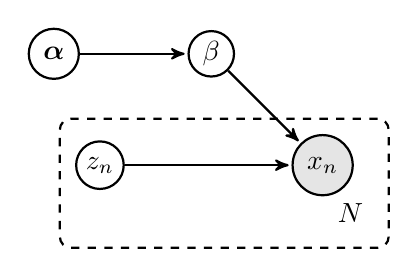
\begin{tikzpicture}[->,>=stealth',shorten >=1pt,auto,node distance=2.5cm,
	  thick,main node/.style={circle,draw,font=\sffamily\normalsize\bfseries, minimum size = 3.5pt}]
	
	  \node[main node] (alpha) {$\boldsymbol{\alpha}$};
	  \node[main node, inner sep=2pt] (beta)  at ($ (alpha) + (0:2) $) {$\beta$};
	  \node[main node, inner sep=2pt] (z_n)  at ($ (beta) + (270-45:2) $) {$z_n$};
	  \node[main node, fill=black!10] (x_n)  at ($ (beta) + (270+45:2) $) {$x_n$};
	  \node [below] (N) at ($ (x_n) + (270+45:0.5) $) {$N$};
	  \node[draw,dashed,fit=(z_n)(x_n)(N), inner sep = 5.5pt, rounded corners] {};

	  \path[every node/.style={font=\sffamily\small}]
	    	(alpha) 	edge 	node [left] 	{} (beta)	    
%	 	(beta)	edge  	node [right] 	{} (z_n)
	 	(beta)	edge  	node [right] 	{} (x_n)
	 	(z_n)	edge  	node [right] 	{} (x_n);
	\end{tikzpicture}

\end{center}

the joint density is of the form:

\begin{equation}\begin{split}
p( \x, \z, \bbeta | \aalpha) &= p(\bbeta|\aalpha) \prod_{n=1}^N p (x_n, z_n | \bbeta)
\end{split}\end{equation}

%where single data likelihood is :
%\begin{equation}\begin{split}
%p( x_n, z_n| x_{-n}, z_{-n}, \bbeta , \aalpha) &= p( x_n, z_n| \bbeta,  \aalpha)
%\end{split}\end{equation}


the conditionals are based on Exponential family:

\begin{equation}\begin{split}
p(\bbeta | \x, \z, \alpha) &= h(\bbeta) \exp \left\{  T(\bbeta)^\top \eta_\post( \x, \z, \alpha) - A_\post( \eta_\post ( \x, \z, \alpha) ) \right\}\\
p(z_{n,j} | x_{n}, z_{n,-j},\bbeta ) &= h(z_{n,j}) \exp\left\{ T (z_{n,j})^\top \eta_{z_{n,j}}(x_n, z_{n,-j},\bbeta)  - A_l \big(\eta_{z_{n,j}}(x_n, z_{n,-j},\bbeta)\big) \right\}\\
\end{split}\end{equation}


Think about why this representation is useful. Let's have a look at a numerical example:

%\vspace{5 mm}
%{\bf Always have in mind } ask yourself where are the {\bf support} of these distributions, i.e., where $p(\x) > 0$?








%-------------------------------------------------------------


\subsubsection{Conjugacy of exponential family distribution}

Let's work through a concrete example of the posterior $p (\bbeta | x_n, z_n)$; instead of writing $\eeta_\beta$, we write $\bbeta$ directly:

\begin{itemize}

\item {\bf prior}:
\begin{equation}\begin{split}
p (\bbeta | \aalpha ) &= h (\bbeta) \exp \{  T(\bbeta)^\top \aalpha- A_\pri (\aalpha)\}\\ 
\end{split}\end{equation}

suppose the sufficient statistics of the {\bf prior} can be written as:

\begin{equation}\begin{split}
T(\bbeta) &=
\begin{bmatrix}
\bbeta \\ {\color{red} -A_l(\bbeta)}
\end{bmatrix}\\
\implies \aalpha &= 
\begin{bmatrix}
\aalpha_1 \\ \alpha_2
\end{bmatrix}
\end{split}\end{equation}

note that $\aalpha_1$ has the same dimensionality as $\bbeta$, and $\alpha_2$ is a scalar quantity. Then the prior itself can be written as:

\begin{equation}\begin{split}
p (\bbeta) &= h (\bbeta) \exp \left\{\begin{bmatrix} \bbeta \\ {\color{red} - A_l(\bbeta)} \end{bmatrix}^\top \;
\begin{bmatrix} \aalpha_1 \\ \alpha_2  \end{bmatrix}  - A_{\pri} (\aalpha) \right\}\\
\end{split}\end{equation}

\item {\bf likelihood}:

and if the likelihood density of $(x_n, z_n)$ can be defined as:

\begin{equation}\begin{split}
p(x_n, z_n | \bbeta ) = h(x_n,z_n) \exp\Big\{  T ( x_n, z_n)^\top \bbeta \; {\color{red} - A_l(\bbeta)} \Big\} \\
\end{split}\end{equation}

\item then {\bf posterior} condition on a single data point:

\begin{equation}\begin{split}\label{eq posterior of beta}
p(\bbeta | x_n, z_n, \aalpha) &\propto \underbrace{h (\bbeta) \exp \{ T(\bbeta)^\top \aalpha  \}} \; \underline{\exp\{  T ( x_n, z_n)^\top \bbeta - A_l (\bbeta) \}}  \quad\quad \because h(x_n,z_n) \text{ is a constant}\\
&= \underbrace{h (\bbeta) \exp \left\{\begin{bmatrix} \bbeta \\ {\color{red} - A_l(\bbeta)} \end{bmatrix}^\top \;
\begin{bmatrix} \aalpha_1 \\ \alpha_2  \end{bmatrix}  - A_{\pri} (\aalpha) \right\}}
\; \underline{\exp\{  T ( x_n, z_n)^\top \bbeta - A_l (\bbeta) \}}  \\
%---------------------------------------------------
&\propto h (\bbeta) \exp \left\{\begin{bmatrix} \bbeta \\ {\color{red} - A_l(\bbeta)} \end{bmatrix}^\top \;
\begin{bmatrix} \aalpha_1 \\ \alpha_2  \end{bmatrix} \right\}
\; \underline{\exp\{  T ( x_n, z_n)^\top \bbeta - {\color{red}A_l (\bbeta)} \}}  \quad\quad \because A_{\pri} (\aalpha) \text{ is a constant}\\
%---------------------------------------------------
&= h (\bbeta) \exp \big\{ \bbeta^\top \aalpha_1  - \alpha_2 {\color{red}A_l(\bbeta)} +  \bbeta^\top T ( x_n, z_n)  - {\color{red} A_l (\bbeta)}  \big\}  \\
%---------------------------------------------------
% &= h (\bbeta) \exp \big\{ \bbeta^\top ( \aalpha_1 +  T ( x_n, z_n) )  - \alpha_2 A_l(\bbeta) - A_l (\bbeta)  \big\}  \\
%---------------------------------------------------
&= h (\bbeta) \exp \big\{ \bbeta^\top \big( \aalpha_1 +  T ( x_n, z_n) \big) - (\alpha_2  + 1 ) {\color{red}A_l(\bbeta)}  \big\}  \\
%---------------------------------------------------
&= h (\bbeta) \exp \bigg\{ \begin{bmatrix} \bbeta \\ {\color{red}  - A_l(\bbeta)}\end{bmatrix}^\top \;  \begin{bmatrix} \aalpha_1 +  T ( x_n, z_n)  \\ \alpha_2  + 1 \end{bmatrix}  \bigg\}  \\
%---------------------------------------------------
&= h (\bbeta) \exp \bigg\{ T(\bbeta)^\top \; \begin{bmatrix} \aalpha_1 +  T ( x_n, z_n)  \\ \alpha_2  + 1 \end{bmatrix}  \bigg\}  \\
\end{split}\end{equation}

notice the posterior ``inherited'' $h(\bbeta)$ from the prior, so we only need to make sure that the $T(\bbeta)$ are the same for both prior and posterior.

\end{itemize}


\subsubsection{posterior over $n$ data points}

% \begin{equation}\begin{split}
% p(\bbeta | \x, \z, \aalpha) &\propto 
% h (\bbeta) \exp \left\{  \begin{bmatrix} \bbeta   \\ - A_l (\bbeta) \end{bmatrix}^\top \begin{bmatrix} \hat{\aalpha}_1 \\ \hat{\alpha}_2 \end{bmatrix} \right\} \\
% &= h (\bbeta) \exp \bigg\{ T(\bbeta)^\top \; \begin{bmatrix}  \aalpha_1 + \sum_{n=1}^{^N}  T ( x_n, z_n)  \\ \alpha_2  + N \end{bmatrix} \bigg\}  \\
% \end{split}\end{equation}

% let's see how we may derive the above expression:


%------------------------------------------------------------------------


\begin{enumerate}
\item {\bf Complete likelihood}

\begin{equation}\begin{split}
p(\x, \z | \bbeta ) &= \prod_{n=1}^{N} \Big\{ h(x_n,z_n) \exp\{ \bbeta^\top T ( x_n, z_n) - A_l (\bbeta) \} \Big\} \\
&= \prod_{n=1}^{N} h(x_n,z_n) \prod_{n=1}^{N} \exp\{ \bbeta^\top T ( x_n, z_n) - A_l (\bbeta) \}  \\
&= h(\x,\z) \exp\left\{ \sum_{n=1}^{N} \bbeta^\top T ( x_n, z_n) - N \times A_l (\bbeta) \right\} \\
\end{split}\end{equation}

\item {\bf Complete posterior}

now, look at:

\begin{equation}\begin{split}
p(\bbeta | \x, \z, \aalpha) 
&\propto h (\bbeta) \exp \left\{\begin{bmatrix} \bbeta \\ {\color{red} - A_l(\bbeta)} \end{bmatrix}^\top \;
\begin{bmatrix} \aalpha_1 \\ \alpha_2  \end{bmatrix} \right\}
\; \underline{\exp\left\{ \sum_{n=1}^{N} \bbeta^\top T ( x_n, z_n) - N \times A_l (\bbeta) \right\}}\\
%---------------------------------------------------
&= 
h (\bbeta) \exp \bigg\{ \begin{bmatrix} \bbeta \\ {\color{red} - A_l(\bbeta)} \end{bmatrix}^\top \; \underbrace{\begin{bmatrix}  \aalpha_1 + \sum_{n=1}^{N}  T ( x_n, z_n)  \\ \alpha_2  + N \end{bmatrix}}_{\eta_\post(\x,\z,\aalpha)} \bigg\}  \\
\end{split}\end{equation}


%\begin{equation}\begin{split}
%p(\bbeta | x_n, z_n, \aalpha) &\propto h (\bbeta) \exp \{ \begin{bmatrix} \alpha_1 +  T ( x_n, z_n)  & \alpha_2  + 1 \end{bmatrix} T(\bbeta)  \}\\
%\implies p(\bbeta | \x, \z, \alpha) &\propto h (\bbeta) \exp \Big\{ \begin{bmatrix} \alpha_1 + \sum_{n=1}^{N}  T ( x_n, z_n)  & \alpha_2  + N \end{bmatrix} T(\bbeta)  \Big\}  \\
%\end{split}\end{equation}

Now we use the expression with $\eta_\post (\x,\z,\aalpha) $ instead:

\begin{equation}\begin{split}
p(\bbeta | \x, \z, \aalpha) &= h (\bbeta) \exp \big\{ \eta_\post (\x,\z,\aalpha)^\top T(\bbeta) - A_\post (\eta_\post (\x, \z, \aalpha)) \big\}\\
\implies  \eta_\post (\x,\z,\aalpha) &= \begin{bmatrix} \aalpha_1 +\sum_{n=1}^{N}  T ( x_n, z_n)  \\ \alpha_2  + N \end{bmatrix}\\
\implies \exp \big( A_\post (\eta_\post (\x, \z, \aalpha)) \big) &= \int_{\bbeta} h (\bbeta) \exp \big\{ \eta_\post (\x,\z,\aalpha)^\top T(\bbeta) \big\} \d \bbeta
\end{split}\end{equation}


\end{enumerate}





%------------------------------------------------------------------------

\subsubsection{Example: Posterior of Gaussian mean}

 
%\subsubsection{likelihood}

suppose data $x_i$ come from a unit variance Gaussian. Compared with Section (\ref{sec Gaussian: Natural Parameter Representation}), we save one parameter:

\begin{equation}\begin{split}
p( x | \mu ) &= \frac{1}{\sqrt{2 \pi}} \exp \Big\{  -\frac{ 1}{2 } ( x - \mu)^2   \Big\} \\
&= \underbrace{\frac{\exp \left( - x^2/2   \right) }{\sqrt{2 \pi}  }}_{h(x)} \exp \Big\{ \underbrace{\mu}_{\beta} \underbrace{x}_{T(x)} - \underbrace{ \frac{ \mu^2}{2 }}_{A_l(\beta)}  \Big\} \\
\end{split}\end{equation}

Therefore:

\begin{equation}\begin{split}
\beta &= \mu\\
T(x)  &= x\\
A_l(\beta) &= \frac{\beta^2}{2}\\
h(x) &= \frac{\exp \left( - x^2/2   \right) }{\sqrt{2 \pi} }
\end{split}\end{equation}

substitute into:

\begin{equation}\begin{split}
p( x | \beta ) 
%&= \frac{\exp \left( - x^2/2   \right) }{\sqrt{2 \pi} } \exp \Big\{ \mu x -  \frac{ \mu^2}{2 }  \Big\}\\
&=  \frac{\exp \left( - x^2/2   \right) }{\sqrt{2 \pi} } \exp \Big\{ \beta x  + \underbrace{ {\color{red}-  \frac{ \beta^2}{2 }}}_{-A_l(\beta)}  \Big\}
\end{split}\end{equation}


\subsubsection{criteria for conjugate pair}



A {\bf conjugate prior} MUST be: 

\begin{equation}\begin{split}\label{eq conjugate prior for variance one Gaussian}
p (\beta | \alpha) &= h (\beta) \exp \Big\{   \alpha_1 \beta   + \alpha_2 ( \underbrace{- \beta^2/2}_{A_l(\beta)} )   - A_g (\alpha)	\Big\}\\
&= h (\beta) \exp \Big\{   \begin{bmatrix}  \alpha_1 \\ \alpha_2\end{bmatrix}^\top \; \begin{bmatrix}  \beta   \\   {\color{red}-\frac{\beta^2}{2}} \end{bmatrix}  - A_g (\alpha) \Big\}
\end{split}\end{equation}

Wait, this doesn't look exactly in the form of Eq.(\ref{eq Gaussian: Natural Parameter Representation}), i.e.,:

\begin{equation}\begin{split}
\N(x; \mu, \sigma^2)  &= \exp \Bigg(   \begin{bmatrix} \frac{ \mu}{ \sigma^2}  \\ - \frac{1}{ 2 \sigma^2}   \end{bmatrix} ^\top \; \begin{bmatrix} x \\ x^2   \end{bmatrix}
 - \frac{\mu^2}{ 2 \sigma^2} - \frac{1}{2} \log ( 2 \pi \sigma^2) \Bigg)\\
\end{split}\end{equation}

We can rearrange Eq.(\ref{eq conjugate prior for variance one Gaussian}) to look like it, but with parameter $\begin{bmatrix}\alpha_1  & -\frac{\alpha_2}{2}  \end{bmatrix}^\top$:


\begin{equation}\begin{split}
p (\beta | \alpha) &= h (\beta) \exp \left\{
\begin{bmatrix}\alpha_1  \\ -\frac{\alpha_2}{2}  \end{bmatrix} ^\top \; \begin{bmatrix} \beta \\ \beta^2   \end{bmatrix}  - A_g (\alpha)	\right\}
\end{split}\end{equation}

From our knowledge, a distribution with sufficient statistics $T(\beta) = \begin{bmatrix} \beta  & \beta^2 \end{bmatrix} $ is a Gaussian distribution.

\vspace{2mm}

Suppose the likelihood is an exponential family distribution. Every exponential family has a conjugate prior in theory. The natural parameter $\aalpha = \begin{bmatrix} \aalpha_1 & \alpha_2 \end{bmatrix}^\top$ has dimension dim$(\bbeta)$ + 1. The sufficient statistics of the prior are $\begin{bmatrix} \bbeta & -A_l(\bbeta)\end{bmatrix}^\top$.









%------------------------------------------------------------------------

\subsection{Conjugate exponential family distribution: $\E_q [ T(\beta) ] = \DLambda A_g(\lambda)$ \optional}


\begin{lemma}

	Given that the exponential family distribution $q(\beta | \lambda)$ is of the form:
	
	\begin{equation}\begin{split}
		q (\beta | \lambda) &= h (\beta) \exp \{ \lambda^\top T(\beta) - A_g (\lambda)\}\\ 
		&= \frac{1}{\exp(A_g (\lambda))} h (\beta) \exp \{ \lambda^\top T(\beta) \}\\
	\end{split}\end{equation}
		
 then the expectation of the sufficient statistics $T(\beta)$ is:		
		\begin{equation}\begin{split}
		\E_{q(\beta)} [ T(\beta) ] = \DLambda A_g(\lambda)
		\end{split}\end{equation}
			
\end{lemma}

proof:

\begin{equation}\begin{split}
&\int_{\beta} q (\beta | \lambda) \d \beta =  \int_{\beta}  h (\beta) \exp \{ \lambda^\top T(\beta) - A_g (\lambda) \} \d \beta = 1\\
&\implies  \DLambda \left( \int_{\beta}  h (\beta) \exp \{ \lambda^\top T(\beta) - A_g (\lambda) \} \d \beta \right) = \DLambda (1) = 0\\
&\implies \int_{\beta}    \DLambda \left( h (\beta) \exp \{ \lambda^\top T(\beta) - A_g (\lambda) \} \right) \d \beta  = 0\\
&\implies \int_{\beta}   h (\beta) \exp \big\{ \lambda^\top T(\beta) - A_g (\lambda) \big\}  \left(   T(\beta) -  \DLambda A_g (\lambda) \right) \d \beta  = 0\\
&\implies \underbrace{\int_{\beta}  h (\beta) \exp \big\{ \lambda^\top T(\beta) - A_g (\lambda) \big\} T(\beta) \d \beta }_{\E_{q(\beta)}[ T(\beta)]}  -
\underbrace{\int_{\beta}  h (\beta) \exp \big\{ \lambda^\top T(\beta) - A_g (\lambda) \big\} \d \beta}_{=1}  \DLambda A_g (\lambda)  = 0\\
&\implies  \E_{q(\beta)}[ T(\beta)]  - \DLambda A_g(\lambda)  = 0
\end{split}\end{equation}





%------------------------------------------------------------------------

\subsubsection{The choice of $q(\beta, \z)$}


We choose $q(\beta, \z)$ to decouple $\beta$ and $\z$ completely:

\begin{equation}
\begin{split}
	q (\beta, \z) = q(\beta | \lambda) \prod_{n=1}^N \prod_{j=1}^J q (z_{n,j} | \phi_{n,j}) 
\end{split}
\end{equation}

 

\begin{itemize}
\item
$q (\beta | \lambda)$ is the SAME distribution type as $p(\beta | \x, \z, \alpha)$, they only differ in parameter. This means they have the same sufficient statistics $T(\beta)$:

\begin{equation}
\begin{split}
	q (\beta | \lambda) &= h (\beta) \exp \{ \lambda^\top T(\beta) - A_g (\lambda)\}\\
\text{compare with:} \hspace{5 mm} 
p(\beta | \x, \z, \alpha) &= h(\beta) \exp \left\{ \eta_\post( \x, \z, \alpha)^\top T(\beta) - A_\post( \eta_\post ( \x, \z, \alpha) ) \right\}\\
\end{split}
\end{equation}

\item
$q (z_{n,j} | \phi_{n,j} )$ is the SAME distribution type as $p(z_{n,j} | x_n, z_{n,-j}, \beta )$, they only differ in parameter. This means they have the same sufficient statistics $T(z_{n,j})$:

\begin{equation}
\begin{split}
	q (z_{n,j} | \phi_{n,j} ) &= h(z_{n,j}) \exp\left\{ \phi^\top_{n,j} T(z_{n,j}) - A_l (\phi_{n,j}) \right\}\\
\text{compare with:} \hspace{5 mm} 
p(z_{n,j} | x_{n}, z_{n,-j},\beta ) &= h(z_{n,j}) \exp\left\{ \eta_l(x_n, z_{n,-j},\beta)^\top T(z_{n,j}) - A_l(\eta_l(x_n, z_{n,-j},\beta)) \right\}\\
\end{split}
\end{equation}

\end{itemize}


%------------------------------------------------------------------------

\subsection{Proof for  $\text{ELBO}(\lambda) $ for $q (\beta | \lambda)$ \optional}

this section shows the proof for the update formula used in Eq.(\ref{eq exponential family update}), i.e., $\eta_j =  \E_{q(\z \setminus z_j | \cdot)} [\eta_\post (\z \setminus z_j )]$, we will do so using an example from the setting described in this section.


Our goal is to maximize the ELBO, i.e., 

\begin{equation}\begin{split}
\text{ELBO}(q) \triangleq \E_{q(\beta, \z)} [\log p (\x, \z, \beta | \alpha )] - \E_{q(\beta, \z)} [\log q(\z, \beta)]\\
\end{split}\end{equation}

Note that $q$ used here is $q(\beta, \z)$, not just $q(\beta | \lambda)$.

\begin{equation}\begin{split}
\text{ELBO}( \lambda)
&= \E_{q(\beta, \z)} [\log p (\beta | \x, \z, \alpha )] + \E_{q(\beta, \z)} [\log p (\x, \z | \alpha)] - \E_{q(\beta, \z)} [\log q(\beta)] \\
	&= \E_{q(\beta, \z)} \big[\log p (\beta | \x, \z, \alpha )\big] - \E_{q} \big[\log q(\beta)\big]+\C \\
&= \E_{q(\beta, \z)} \left[\log \big(  h (\beta) \exp \big\{ \eta_\post (\x,\z,\alpha)^\top T(\beta) - A_\post (\eta_\post (\x,\z, \alpha)) \big\}  \big) \right] - {\color{red}\E_{q} [\log q(\beta)]}+\C \\
%---------------------------------------------------
&= \E_{q(\beta, \z)} [\log (h (\beta))] +  \underline{\E_q [ \eta_\post (\x,\z,\alpha)^\top T(\beta) ]} 
   - {\color{red}\E_{q} \big[\log \big( h (\beta) \exp \{ \lambda^\top T(\beta) - A_\pri (\lambda)\} \big) \big]}+\C \\
%---------------------------------------------------
&= \underbrace{\E_{q(\beta, \z)} [\log (h (\beta))]}_{\text{doesn't contain } \lambda} +\underline{\E_{q(\z|\Phi)} [\eta_\post (\x,\z,\alpha)]^\top  \E_{q (\beta | \lambda)} [  T(\beta) ]} 
   - \underbrace{\E_{q(\beta, \z)} [\log  h (\beta)]}_{\text{doesn't contain } \lambda} - \E_q [ \lambda^\top T(\beta) ]+  A_\pri (\lambda) + \C \\
%---------------------------------------------------
&=  \E_{q(\z|\Phi)} [\eta_\post (\x,\z,\alpha)]^\top \E_{q(\beta |\lambda)} [  T(\beta) ] - \lambda^\top \E_{q(\beta|\lambda)} [  T(\beta) ]+  A_\pri (\lambda) + \C \quad\quad \because A_\pri (\lambda) \text{ contains } \lambda\\
\end{split}\end{equation}

now let's substitute $\E_{q(\beta|\lambda)} [ T(\beta) ] = \DLambda A_\pri(\lambda)$ into \text{ELBO}$(\lambda)$:

\begin{equation}\begin{split}
\text{ELBO}(\lambda) &= \E_{q(\z|\Phi)} [\eta_\post (\x,\z,\alpha)]^\top  \DLambda A_\pri(\lambda) {\color{red}- \lambda^\top  \DLambda A_\pri(\lambda)} + A_\pri (\lambda) + \C \\
\end{split}\end{equation}


%------------------------------------------------------------------------

%\subsection{Update for $\L(\lambda)$}
%\begin{equation}
%\begin{split}
%	\L(\lambda) &= \E_{q(Z|\Phi)} [\eta_g (x,z,\alpha)]^\top  \DLambda A_g(\lambda) - \lambda^\top  \DLambda A_g(\lambda) + A_g (\lambda) + \C \\
%\end{split}
%\end{equation}

Maximize $\text{ELBO} (\lambda)$ we get:

\begin{equation}\begin{split}
\DLambda \text{ELBO}(\lambda) &= \E_{q(\z|\Phi)} [\eta_\post (\x,\z,\alpha)]^\top  \nabla^2_{\lambda} A_\pri(\lambda) {\color{red} - \DLambda A_\pri(\lambda) -  \lambda^\top \DLambda^2 A_\pri(\lambda)} + \DLambda A_\pri (\lambda) = 0 \\
&= \E_{q(\z|\Phi)} [\eta_\post (\x,\z,\alpha)]^\top  \nabla^2_{\lambda} A_\pri(\lambda) -  \lambda^\top \DLambda^2 A_\pri(\lambda) = 0 \\
&\implies  \nabla^2_{\lambda} A_\pri(\lambda) \big( \E_{q(\z|\Phi)} [\eta_\post (\x,\z,\alpha)]^\top   -  \lambda^\top \big) = 0 \\
\end{split}\end{equation}


\begin{equation}\begin{split}
\lambda =  \E_{q(\z|\Phi)} [\eta_\post (\x, \z,\alpha)]
\end{split}\end{equation}


in words, when we try to update $\lambda$ for $q(\beta | \lambda)$, we find the corresponding posterior $p (\beta | \x, \z, \alpha )$, and its natural parameter $\eta_\post (\x, \z,\alpha)$, then compute the expectation with all the $q(\cdot)$ that its natural parameter has random variables for.


%------------------------------------------------------------------------

\subsection{Update for $\text{ELBO}(\phi_{n,j})$ for $q(z_{n,j} | \phi_{n,j})$ \optional}

 

In a very similar fashion to $\text{ELBO}(\lambda)$, we can prove:

\begin{equation}\begin{split}
	\DPhi \text{ELBO}(\phi_{n,j}) &=  \nabla^2_{\phi_{n,j}} A_l(\phi_{n,j}) \big( \E_{q(\lambda)} [\eta_l (x_n, z_{n,-j},\beta)]^\top   - \phi_{n,j}^\top \big) = 0 \\
\end{split}\end{equation}



\begin{equation}\begin{split}
 \phi_{n,j} =  \E_{q(\lambda)} \big[\eta_l(x_n,z_{n,-j}, \beta)\big]
\end{split}\end{equation}

in words, when we try to update $ \phi_{n,j} $ for $q(z_{n,j} | \phi_{n,j})$, we find the corresponding posterior $p ( z_{n,j} | x_n, z_{n,-j} )$, and its natural parameter $\eta_l (x_n, z_{n,-j})$, then compute the expectation with all the $q(\cdot)$ that its natural parameter has random variables for.

\newpage



%------------------------------------------------------------------------

%\subsection{Continue next time for Stochastic Maximization \dots}





%------------------------------------------------------------------------

\section{apply variational inference (Exponential family version) to Latent Dirichlet Allocation \optional}

let's visit Latent Dirichlet Allocation again \cite{blei2003latent}:

\begin{center}
	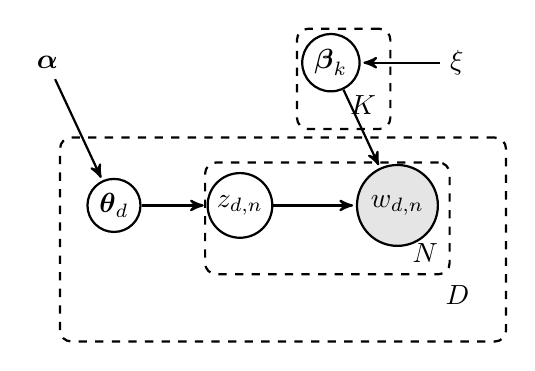
\begin{tikzpicture}[->,>=stealth',shorten >=1pt,auto,node distance=2.5cm,
	  thick,main node/.style={circle,draw,font=\sffamily\normalsize\bfseries, minimum size = 3.5pt}]
	
	  \node (alpha) {$\boldsymbol{\alpha}$};
	  \node[main node, inner sep=2pt] (theta)  at ($ (alpha) + (270+25:2) $) {$\ttheta_d$};
	  \node[main node, inner sep=2pt] (beta)  at ($ (alpha) + (0:3.6) $) {$\bbeta_k$};
	  \node (xi)  at ($ (beta) + (0:1.6) $) {$\xi$};
	  \node[main node, inner sep=2pt] (z)  at ($ (theta) + (0:1.6) $) {$z_{d,n}$};
	  \node[main node, fill=black!10] (w)  at ($ (beta) + (270+25:2) $) {$w_{d,n}$};
	  \node [below] (N) at ($ (w) + (270+45:0.5) $) {$N$};
	  \node [below] (D) at ($ (N) + (270+55:0.5) $) {$D$};
	  \node [below] (K) at ($ (beta) + (270+55:0.5) $) {$K$};
	  \node[draw,dashed,fit=(beta)(K), inner sep = 1.5pt, rounded corners] {};
	  \node[draw,dashed,fit=(z)(w)(N), inner sep = 0.5pt, rounded corners] {};
	  \node[draw,dashed,fit=(theta)(z)(N)(w)(D), inner sep = 9.5pt, rounded corners] {};

	  \path[every node/.style={font=\sffamily\small}]
	    	(alpha) 	edge 	node [left] 	{} (theta)	    
	 	(theta)	edge  	node [right] 	{} (z)
	 	(beta)	edge  	node [right] 	{} (w)
	 	(xi)	edge  	node [right] 	{} (beta)
	 	(z)	edge  	node [right] 	{} (w);
	\end{tikzpicture}
\end{center}


\begin{itemize}

\item
$\bbeta_k \sim \text{Dir} (\xi, \dots, \xi)$ for $k \in \{1,...,K\}$.

\item 
For each document $d$:\\
\hspace{5 mm} $\ttheta_d \sim \text{Dir} ( \alpha, \dots, \alpha)$\\
\hspace{5 mm} For each word $w \in \{1,...,N\}$:\\
\hspace{10 mm} $z_{dn} \sim \text{Mult} (\ttheta_d)$\\
\hspace{10 mm} $w_{dn} \sim \text{Mult} (\bbeta_{z_{dn}})$


\end{itemize}



\subsection{define corresponding $q(\cdot)$}


\begin{enumerate}
\item $q(z_{d,n})$ 

\begin{equation}\begin{split}
q(z_{d,n}) &= \text{Mult}(\pphi_{d,n})\\
\implies q(z_{d,n} = k) &= \phi^k_{d,n}
\end{split}\end{equation}

\item $q(\bbeta_k) $

\begin{equation}\begin{split}
q(\bbeta_k) = \text{Dir} (\llambda_k)
\end{split}\end{equation}


\item $q(\ttheta_d)$

\begin{equation}\begin{split}
q(\ttheta_d)= \text{Dir}(\ggamma_d)
\end{split}\end{equation}


\end{enumerate}

\subsubsection{Facts about Dirichlet Distribution}


\begin{equation}\begin{split}
\theta &\sim \text{Dir} (\gamma_1, \dots \gamma_K)\\ 
\implies  \E [ \log(\theta_k) | \gamma] &=  \Psi(\gamma_k) - \Psi \bigg( \sum_{i=1}^{K}  \gamma_i  \bigg)\quad\text{for component } k
\end{split}\end{equation}

where: 

\begin{equation}\begin{split}
\Psi (x)= \frac {\mathrm {d} }{\mathrm {d} x}\ln \big (\Gamma (x) \big )=\frac {\Gamma '(x)}{\Gamma (x)}
\end{split}\end{equation}



%------------------------------------------------------------------------

\subsection{Updating $q(z_{d,n} | \pphi_{d,n})$: optimize $\pphi_{d,n}$}

\subsubsection{find natural parameter of posterior $p(z_{dn} = k | \ttheta_d, \bbeta_{1:K},w_{d,n} ) $}


\begin{equation}\begin{split}
p(z_{d,n} = k | \ttheta_d, \bbeta_{1:K},w_{d,n} ) &\propto  p(z_{d,n} = k | \ttheta_d) p(w_{d,n} | z_{d,n} = k , \bbeta_{1:K} ) \\
&= \theta_{d, k} \times  \beta_{k, w_{d,n}} \\
&\propto \exp \bigg( \underbrace{\log(\theta_{d,k}) +\log(\beta_{k,w_{d,n}})}_{\eta_l \left(\ttheta_d, \bbeta_{1:K}, w_{d,n} \right)}  \times \underbrace{1}_{T(z_{d,n})}\bigg)\\
\end{split}\end{equation}

for the last line, we substitute the exponential family form of the multinomial distribution. Expressing it using the ``normal'' multinomial distribution, its parameter is:


\begin{equation}\begin{split}
p(z_{d,n} | \ttheta_d, \bbeta_{1:K},w_{d,n} )
&=
\text{Mult}\big(
\theta_{d, 1} \times  \beta_{1, w_{d,n}}, \dots, \theta_{d, K} \times  \beta_{K, w_{d,n}} \big)
\end{split}\end{equation}

diagrammatically, $\bbeta_{1:K}$ is represented as a matrix of:

\begin{equation}\begin{split}
\bbeta_{1:K} \equiv \begin{bmatrix}
-- & \bbeta_1 & --\\
\vdots & \vdots & \vdots\\
-- & \bbeta_K & --\\
\end{bmatrix}
\equiv \begin{bmatrix}
\beta_{1,w_1}& \dots & \beta_{1,w_{|\mathcal{V}|}}\\
\vdots & \vdots & \vdots\\
\beta_{K,w_1}& \dots & \beta_{K,w_{|\mathcal{V}|}}\\
\end{bmatrix}
\end{split}\end{equation}



\subsubsection{optimize $\pphi_{d,n}$}


apply the update formula, in which we need the natural parameter for $p(z_{d,n} | \ttheta_d, \bbeta_{1:K}, w_{d,n} )$ in the expectation:

\begin{equation}\begin{split}
\eta( \phi^k_{d,n} ) = \log( \phi^k_{d,n} ) &\propto \E_{q(\ttheta_d)q(\bbeta_k) } \left[ \eta_l \left(\ttheta_d, \bbeta_{1:K}, w_{d,n} \right) \right]\\
&= \E_{q(\ttheta_d, \bbeta_{1:K})} \left[ \log(\theta_{d,k}) \right] +  \E_{q(\bbeta_k)}  \left[  \log(\beta_{k,w_{d,n}}) \right]\\ 
&= \Psi(\gamma_{d,k}) - \Psi \Big( \sum_{k=1}^K \gamma_{d,k}  \Big) +  \Psi \Big( \lambda_{k, w_{d,n}} \Big) - \Psi \Big( \sum_{v} \lambda_{k,v}  \Big) \\
\end{split}\end{equation}

compare this with Eq.(\ref{eq exponential family update}), i.e., $\eta_j =  \E_{q(\z \setminus z_j )} [\eta_\post (\z \setminus z_j )]$, you can see easily that: 

\begin{equation}\begin{split}
\z \setminus z_j &\equiv \{ \ttheta_d, \bbeta_{1:K} \}
\end{split}\end{equation}





to obtain $\pphi_{d,n}$:

\begin{equation}\begin{split}
\implies \phi^k_{d,n} &\propto  
\exp \Bigg[ \Psi(\gamma_{d,k}) - \Psi \Big( \sum_{k=1}^K \gamma_{d,k}  \Big)+  \Psi \Big( \lambda_{k, w_{d,n}} \Big) - \Psi \Big( \sum_{v} \lambda_{k,v}  \Big) \Bigg] \\
&\propto \exp \bigg[ \Psi(\gamma_{d,k}) +  \Psi \Big( \lambda_{k, w_{d,n}} \Big) - \Psi \Big( \sum_{v} \lambda_{k,v}  \Big) \bigg] \quad
\because \sum_{k=1}^K \gamma_{d,k}  \text{ has the same value irrespective of } k\\
\end{split}\end{equation}



%------------------------------------------------------------------------

\subsection{Updating $q(\ttheta_d | \ggamma_d )$: optimize $\ggamma_d$}

\subsubsection{find natural parameter of posterior $p( \ttheta_d | \z_{d} )$}


\begin{equation}\begin{split}\label{eq posterior of theta d}
p( \ttheta_d | \z_{d} ) &\propto p(\ttheta_d | \aalpha) \prod_{n=1}^N  p(z_{d,n} | \ttheta_d)
= \text{Dir} (\aalpha) \times \prod_{n=1}^N \text{Mult} ( z_{d,n} | \ttheta_d)\\ 
%-------------------------
&= \prod_{k} \Big( \theta_{d,k}^{\alpha_k - 1} \prod_{n=1}^{N} \theta_{d,k}^{\1(z_{d,n}= k)} \Big) \\
%------------------------
&= \exp\Big[  \log \Big( \prod_{k} \Big( \theta_{d,k}^{\alpha_k - 1} \prod_{n=1}^{N} \theta_{d,k}^{\1(z_{d,n}= k)} \Big)  \Big) \Big]\\
%-------------------------
&= \exp\left[  \sum_{k}  \log  \Big( \theta_{d,k}^{\alpha_k - 1} \prod_{n=1}^{N} \theta_{d,k}^{\1(z_{d,n}= k)} \Big)   \right]\\
&= \exp\left[  \sum_{k}   \left(  \log \theta_{d,k}^{\alpha_k - 1} +  \sum_{n=1}^{N} \log \left( \theta_{d,k}^{\1(z_{d,n}= k)} \right) \right)   \right]  \\
%-------------------------
&= \exp\left[  \sum_{k}   \left(  (\alpha_k - 1) \log \theta_{d,k} +  \sum_{n=1}^{N} \1(z_{d,n} =  k) \log  \theta_{d,k}  \right)   \right]  \\
%-------------------------
&= \exp\left[  \sum_k  \left( \alpha_k - 1 + \sum_{n=1}^{N} \1(z_{d,n} =  k) \right)  \log \left(   \theta_{d,k}   \right) \right]\\
%-------------------------
=& \exp\Bigg( \underbrace{\begin{bmatrix} (\alpha_1 - 1 + n_1) \\ \dots \\ (\alpha_K - 1 + n_K)  \end{bmatrix}^\top}_{\eta_l \left(\alpha,  z_{d} \right)}  
\underbrace{ \begin{bmatrix} \log(\theta_{d,1}) \\ \dots \\ \log(\theta_{d,K}) \end{bmatrix}}_{T(\ttheta_d)}\Bigg) \quad\quad\text{ by letting } n_k = \sum_{n=1}^N \1( z_{d,n}= k )\\
=&\text{Dir}(\alpha_1 + n_1, \dots, \alpha_K + n_K)\\
\end{split}\end{equation}

It turns out that the Dirichlet distribution is the only distribution with exactly the same ``normal'' and natural parameters.

%\subsubsection{define corresponding $q(\cdot)$}
%\begin{equation}\begin{split}
%q(z_{d,n}) &= \text{Mult}(\pphi_{d,n}) \text{ or } q(z_{d,n} = k) = \phi^k_{d,n}\\
%q(\bbeta_k) &= \text{Dir} (\llambda_k)\\
%q(\ttheta_d) &= \text{Dir}(\ggamma_d)\\
%\end{split}\end{equation}


\subsubsection{optimize $\ggamma_d$}

let's use $q(\eta(\ggamma_d)) = \text{Dir}(\eta(\ggamma_d))$ to approximate $p( \ttheta_d | \z_{d} ) $ (another Dirichlet distribution), we apply the exponential family update formula Eq.(\ref{eq exponential family update}):

\begin{equation}\begin{split}
\eta(\ggamma_d) &= \E_{q(z_{d,n} | \pphi_{d,n} )} \left[ \eta_l \left(\alpha,  z_{d} \right) \right]\\
&= \E_{q(z_{d,n} | \pphi_{d,n} )}   \begin{bmatrix}(\alpha_1 - 1 + n_1) & \dots & (\alpha_K - 1 + n_K)  \end{bmatrix}\quad\text{substitute Eq.(\ref{eq posterior of theta d})}\\
\end{split}\end{equation}

compare this with Eq.(\ref{eq exponential family update}), i.e., $\eta_j =  \E_{q(\z \setminus z_j )} [\eta_\post (\z \setminus z_j )]$, you can see easily that: 

\begin{equation}\begin{split}
\z \setminus z_j &\equiv \{ z_{d,n} \}
\end{split}\end{equation}

how to compute $\E_{q(z_{d,n} | \pphi_{d,n} )}  \big[n_1\big]$? Firstly, let's recognize that $\pphi_{d,n}$ itself is a probability vector:

\begin{equation}\begin{split}\label{eq update for phi d n}
\pphi_{d,n} &=
\begin{bmatrix}
\phi_{d,n}^1 & \dots & \phi_{d,n}^K
\end{bmatrix}\\
&=\begin{bmatrix}
q(z_{d,n} = 1) & \dots & q(z_{d,n} = K)
\end{bmatrix}\\
\end{split}\end{equation}

since:

\begin{equation}\begin{split}
\E\big[\sum_{n=1}^N \1(z_{d,n} =  k) \big]&= \sum_{n=1}^N \E[ \1(z_{d,n} =  k) ]\\
&= \sum_{n=1}^N  q( z_{d,n} =  k)\\
&=  \sum_{n=1}^N  \phi_{d,n}^k
\end{split}\end{equation}

continue with Eq.(\ref{eq update for phi d n}), we have:

\begin{equation}\begin{split}
\eta(\ggamma_d) &= \begin{bmatrix}\alpha_1 - 1 + \sum_{n=1}^N  \phi_{d,n}^1  & \dots &  \alpha_K - 1 + \sum_{n=1}^N  \phi_{d,n}^K \end{bmatrix} \\
%&= \begin{bmatrix}(\alpha_1 - 1 + \sum_{n=1}^N \1(z_{d,n} =  1 ) \phi^1_{d,n} )  & \dots &  (\alpha_K - 1 + \sum_{n=1}^N  \1(z_{d,n} = K ) \phi^K_{d,n}) \end{bmatrix} \\
\end{split}\end{equation}


to obtain the Dirichlet distribution parameter $\ggamma_d$: luckily, for the Dirichlet distribution, the natural and ``normal'' parameters are the same.


\begin{equation}\begin{split}
\ggamma_{d}
&= \begin{bmatrix} \left(\alpha_1 +  \sum_{n=1}^N \phi^1_{d,n} \right) & \dots & \left(\alpha_K + \sum_{n=1}^N  \phi^K_{d,n}  \right) \end{bmatrix} \\
&= \aalpha +  \sum_{n=1}^N \pphi_{d,n}\\
\end{split}\end{equation}



%------------------------------------------------------------------------

\subsection{Updating $q(\bbeta_{k} | \llambda_k)$ optimize $\llambda_k$}


\subsubsection{find natural parameter of posterior $p( \bbeta_{k} | \z, \w )$}

\begin{equation}\begin{split}
p( \bbeta_{k} | \z, \w ) &\propto p(\bbeta_k | \xi) \prod_{d=1}^D \prod_{n=1}^N  p \left(w_{d,n} | \bbeta_{k}\right)^{ \1(z_{d,n}= k)}
= \text{Dir} (\xi) \times  \prod_{d=1}^D \prod_{n=1}^N \beta_{k,w_{d,n}}^{\1(z_{d,n}= k) } \\
&\propto \exp\bigg( \underbrace{\left(   \xi - 1 +  \sum_{d=1}^D \sum_{n=1}^N  w_{d,n}  \1(z_{d,n}= k)    \right)}_{\eta_l \left(\xi,  Z, W \right)}  \times \underbrace{\log(\bbeta_k)}_{T(\bbeta_{k})}\bigg)\\
&=\text{Dir}(\eta_l \left(\xi,  Z, W \right))
\end{split}\end{equation}


%\subsubsection{define corresponding $q(\cdot)$}
%\begin{equation}\begin{split}
%q(z_{d,n}) &= \text{Mult}(\pphi_{d,n}) \text{ or } q(z_{d,n} = k) = \phi^k_{d,n}\\
%q(\bbeta_k) &= \text{Dir} (\llambda_k)\\
%q(\ttheta_d) &= \text{Dir}(\ggamma_d)
%\end{split}\end{equation}



\subsubsection{optimize $\llambda_k$}

let's use $q(\eta(\llambda_k)) = \text{Dir}(\eta(\llambda_k))$ to approximate $p( \bbeta_{k} | \z, \w )$ (another Dirichlet distribution), we apply the exponential family update formula Eq.(\ref{eq exponential family update}):


\begin{equation}\begin{split}
\eta(\llambda_k) &= \E_{\prod_{d=1}^D \prod_{n=1}^N q(z_{d,n} | \phi^k_{d,n})  } \left[ \eta_l (\xi,  \z, \w ) \right]\\
&=  \E_{\prod_{d=1}^D \prod_{n=1}^N q(z_{d,n} | \phi^k_{d,n})  }  \left[ \xi -1 +  \sum_{d=1}^D \sum_{n=1}^N  w_{d,n}  \1(z_{d,n}= k)  \right]\\
&= \xi -1  +  \sum_{d=1}^D \sum_{n=1}^N  w_{d,n} \phi^k_{d,n}  \\
\end{split}\end{equation}



\begin{equation}\begin{split}
\llambda_k &= \xi  +  \sum_{d=1}^D \sum_{n=1}^N  w_{d,n} \phi^k_{d,n}  \\
\end{split}\end{equation}


\newpage







%------------------------------------------------------------------------

\section{Collapsed Variational Inference \optional}


\begin{equation}
\begin{split}
&q(z_{d,n}) = \text{Mult}(\pphi_{d,n}) \text{ or } q(z_{d,n} = k) = \phi^k_{d,n}
\hspace{5 mm} q(\bbeta_k) = \text{Dir} (\llambda_k)
\hspace{5 mm} q(\ttheta_d)= \text{Dir}(\ggamma_d)\\
\end{split}
\end{equation}

\begin{equation}
\begin{split}
\implies q(Z, \ttheta_1\dots \ttheta_D, \bbeta_1 \dots \bbeta_K)
&= \left( \prod_{d=1}^{D} \prod_{n=1}^N q (z_{d,n} | \pphi_{d,n})\right) \prod_{d=1}^{D} q (\ttheta_d | \ggamma_d) \prod_{k=1}^K  q (\bbeta_k| \llambda_k)\\
\text{ now change to:} &=  \underbrace{\left( \prod_{d=1}^{D} \prod_{n=1}^N q (z_{d,n} | \pphi_{d,n})\right)}_{q(Z)}  q({ \Theta}, { \beta} | Z)\\
\end{split}
\end{equation}

Maximizing ELBO, it becomes: (remove $X$ for clarity)


Let $U = \{ \Theta, \beta \}$:

\begin{equation}
\begin{split}
	\text{ELBO}(q) &\triangleq \E_{q( U, Z) } [\log p (Z, U )] - \E_{q( U, Z)} [\log q(Z, U)]\\
	&= \E_{q( U, Z) } [\log p (Z, U )] - \E_{q( U, Z)} [\log q(U | Z) - \log q(Z) ]\\
	&= \E_{q (Z)} \left(  \E_{ q( U | Z) } [\log p (Z, U )]  \right) - \E_{q (Z)} \left(  \E_{ q( U | Z) }  [\log q( U | Z)] \right) -  \E_{q(Z, U)} [\log q(Z)] \\
	&= \E_{q (Z)} \left(  \underbrace{ \E_{ q( U | Z) } \left( [\log p (Z, U )] -  [\log q( U | Z)] \right)}_{\mathcal{L}(q( U | Z)) }  \right)-  \E_{q(Z)} [\log q(Z)] \\
\end{split}
\end{equation}

Think of this as treating $Z$ as $X$.


 

(removed $X$ for clarity)


\begin{equation}\begin{split}
	\argmax_{q( U | Z) } ( \text{ELBO}(q) )
	&=  \argmax_{q( U | Z) } \left[ \E_{q (Z)} \left(  \underbrace{ \E_{ q( U | Z) } \left( [\log p_X (Z, U )] -  [\log q( U | Z)] \right)}_{\mathcal{L}(q( U | Z)) }  \right)-  \E_{q(Z)} [\log q(Z)] \right] \\
		&= \E_{q (Z)} \left(  \underbrace{ \max_{q( U | Z) } \left[  \E_{ q( U | Z) } \left( [\log p (Z, U )] -  [\log q( U | Z)] \right) \right]}_{ }  \right) -  \E_{q(Z)} [\log q(Z)] \\
		&= \E_{q (Z)} [  \underbrace{\log p(Z)} ]-  \E_{q(Z)} [\log q(Z)]  \\
\end{split}\end{equation}

\begin{equation}\begin{split}
 \max_{q( U | Z) } \left[  \E_{ q( U | Z) } \left( [\log p (Z, U )] -  [\log q( U | Z)] \right) \right] = \log p(Z)
\end{split}\end{equation}


the maximum occurs when $q ( U | Z ) = p( U | Z) \implies \KL  \left( q( U | Z)  \| p(U | Z) \right) = 0$

%-------------------------------------------------------------------------


\bibliography{../includes/refs}
\bibliographystyle{../includes/IEEEbib}
\end{document}
